\documentclass[12pt,a4paper,oneside,openright,titlepage]{book}
\usepackage[T1]{fontenc}
\usepackage[utf8]{inputenc}
\usepackage[italian]{babel}
\usepackage{graphicx}
\usepackage{listings}
\usepackage{mathtools}
\usepackage{enumerate}
\usepackage{forest}
\usepackage{booktabs}
\usepackage{caption}
\usepackage{multirow}
\usepackage{amsmath}
\pagestyle{headings}
\definecolor{javapurple}{rgb}{0.5,0,0.35} % keywords
\definecolor{javadocblue}{rgb}{0.25,0.35,0.75} % javadoc
\definecolor{javagreen}{rgb}{0.25,0.5,0.35} % comments
\definecolor{backcolour}{rgb}{0.95,0.95,0.92}%background
\lstset{language=Java,
	aboveskip=3mm,
	belowskip=3mm,
	columns=flexible,
	frame=tb,%single
	keywordstyle=\color{javapurple}\bfseries,
	stringstyle=\color{blue},
	commentstyle=\color{javagreen},
	morecomment=[s][\color{javadocblue}]{/**}{*/},
	numbers=left,%none
	numberstyle=\color{black},
	stepnumber=1,
	numbersep=20pt,
	tabsize=3,
	breaklines=true,
	showspaces=false,
	showstringspaces=false,
	backgroundcolor=\color{backcolour},
	basicstyle=\ttfamily\footnotesize}
\begin{document}
	\frontmatter
	\begin{titlepage}
\begin{center}
	{\LARGE Università degli Studi di Salerno}\par
	\vspace{0.5cm}
	{\Large Dipartimento di Informatica}\par
	\vspace{1cm}
	
\includegraphics[height=160pt]{files/logounisa.png}\par
	\vspace{1cm}
	{\Large Corso di Laurea Magistrale in Informatica}\par
	\vspace{2cm}
	{\Huge GLL Parsing su linguaggi non lineari}\par
	\vspace{2cm}
\end{center}
\begin{flushleft}
	{\large\textbf{Relatore}}
	\hspace{8cm}
	{\large\textbf{Candidato}}\par
	\vspace{0.1cm}
	{\large Prof. Gennaro Costagliola}
	\hspace{4.5cm}
	{\large Mazzotta Fabio}%\\
	%{\normalsize Matr. 0522500518}\par
\end{flushleft}	
	\vspace{3.5cm}
\begin{center}
	{\large Anno Accademico 2019-2020}
\end{center}
\end{titlepage}
	\null\vspace{\stretch{1}}
\begin{flushright}
	\textit{Ai miei genitori.}\par
	\textit{Dedicato a chi ha creduto in me;}\\
	\textit{e a chi lotta ogni giorno e non si arrende.}\par
\end{flushright}
\vspace{\stretch{2}}\null

	\tableofcontents	
	\listoffigures
	\listoftables
	\mainmatter
	\chapter{Introduzione}
\section{Introduzione alla tesi}
Questa tesi di laurea descrive il funzionamento e l'implementazione del parsing \textbf{Generalizzato LL (GLL)} sui linguaggi non lineari. Il parsing GLL è un algoritmo di parsing top down che viene utilizzato per gestire tutte le grammatiche context-free che sono ambigue e ricorsive a sinistra. La caratteristica principale di questo algoritmo è che risulta essere un parser a \textbf{discesa ricorsiva} e ciò permette di avere il controllo del flusso sulle strutture della grammatica e risultano semplici da implementare e semplici da testare passo dopo passo attraverso il debugger. Questo parser è stato utilizzato per riconoscere linguaggi non lineari (bidimensionali) generati da grammatiche posizionali, ossia generalizzazioni di grammatiche context-free. La tesi è divisa in tre parti. Nella prima parte si cerca di illustrare come funziona il parsing LL, che rappresenta la base del parsing GLL, e i suoi limiti. Successivamente si  discuterà come estendere il parsing LL attraverso il parsing GLL, illustrandone i principi e le strutture dati che utilizza. Ciò viene descritto rispettivamente nel secondo e terzo capitolo. Nella seconda parte si analizzaranno le grammatiche posizionali. Questo argomento sarà trattato nel quarto capitolo. Nell'ultima parte si parlerà l'implementazione del parsing GLL applicato ad una grammatica posizionale. In particolare nel quinto capitolo si descriverà le varie  componenti software del parsing GLL, nel sesto capitolo si illustrerà come viene applicato il software del parsing GLL ad una grammatica posizionale e nel settimo capitolo si parlerà del tool utilizzato per testare il software del parsing GLL. Infine nell'ottavo capitolo si discuteranno i risultati ottenuti e gli sviluppi futuri.

	\chapter{Parsing top down}
\section{Introduzione}
Il parsing, o analisi sintattica, è una fase di compilazione  che viene utilizzata per definire la sintassi di un linguaggio di programmazione. In altre parole definisce la struttura corretta di un programma. Utilizza i token \cite{libro: compilatori}, ossia sequenze di caratteri restituite da un analizzatore lessicale (Lexer); per produrre una rappresentazione intermedia ad albero che rappresenta la struttura grammaticale dei token. Il risultato ottenuto dal parsing è l'\textit{albero sintattico}, o \textit{syntax tree}, in cui un nodo interno rappresenta un'operazione mentre i figli rappresentano gli argomenti dell'operazione; infine, questo albero prodotto, viene passato alle restanti fasi del processo di compilazione. Ovviamente, il parser è in grado segnalare gli errori delle forme sintattiche sbagliate. In figura 2.1 viene mostrato il funzionamento del parser.
\par
\vspace{0.5mm}
\begin{figure}[hbpb]\label{figParser}
	{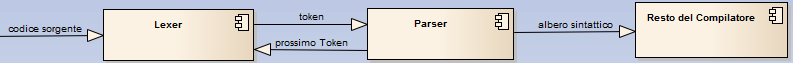
\includegraphics[height=40pt,width=420pt,scale=0.1]{files/parser.png}}
	\caption{\textit{Posizione del parser all'interno del compilatore.}}
\end{figure}
\noindent I metodi di parsing più comunemente utilizzati sono:
\begin{itemize}
	\item \textbf{Parsing top down:} la costruzione dell'albero sintattico avviene partendo dalla radice dell'albero fino ad arrivare alle foglie dell'albero;
	\item \textbf{Parsing bottom up:} la costruzione dell'albero sintattico avviene partendo dalle foglie dell'albero fino ad arrivare alla sua radice.
\end{itemize}
In questa tesi tratteremo il parsing top down in quanto il GLL parsing usa questa metodologia.
\section{Grammatiche context-free}
In questo paragrafo introduciamo le grammatiche context-free. Sono delle notazioni usate per descrivere la sintassi dei costrutti dei linguaggi di programmazione. Ad esempio in C, il while può essere definito con la seguente forma:
\begin{align}
	\textbf{while} \quad (expression) \quad statement \notag
\end{align}
Questa notazione indica che il costrutto è composto dalla parola chiave \textbf{while}, una parentesi tonda aperta, un'espressione, una parentesi tonda chiusa e uno statement. Usando la variabile \textit{expr} che indica una generica espressione e la variabile \textit{stmt} per indicare lo statement, la regola di questo costrutto può essere definita nel seguente modo:
\begin{align}\label{regolaWhile}
	stmt \to \textbf{while } ( expr ) \quad stmt 
\end{align}
La freccia può essere letta come "può avere la forma". Questa regola prende il nome di \textbf{produzione. }All'interno della produzione la parola \textit{while}, la parentesi aperta e tonda prendono il nome di \textbf{terminali}, mentre le variabili \textit{expr} e \textit{stmt} prendono il nome di \textbf{non-terminali}.
\subsection{Definizione di grammatica}
Una grammatica context-free è una quadrupla i cui elementi sono \cite{libro: compilatori}:
\begin{enumerate}
	\item \textbf{Terminali. }I terminali sono simboli di base con cui la grammatica definisce il linguaggio. Il termine "\textit{token}" è un sinonimo di terminale.
	\item \textbf{Non-Terminali. }I non-terminali sono variabili sintattiche che denotano un insieme di stringhe. Nella produzione \ref{regolaWhile} \textit{stmt} e \textit{expr} sono non-terminali. Gli insiemi di stringhe rappresentati dai non-terminali concorrono a definire il linguaggio generato dalla grammatica.
	\item \textbf{Simbolo Iniziale. }In una grammatica uno dei non-terminali costituisce il simbolo iniziale e l'insieme di stringhe che esso denota coincide con l'intero linguaggio generato dalla grammatica. 
	\item \textbf{Produzione. }Le produzioni di una grammatica definiscono come i terminali e i non-terminali possono essere combinate a formare stringhe. Ogni produzione è formata da:
	\begin{enumerate}[(a)]
		\item un non-terminale chiamato \textbf{testa}; la produzione definisce alcune delle stringhe denotate alla sua testa;
		\item il simbolo $\to$; a volte il simbolo $\Coloneqq$ è utilizzato al posto della freccia;
		\item un \textbf{ corpo } o \textbf{lato destro} costituito da zero o più non-terminali o terminali; i componenti descrivono un modo in cui le stringhe denotate dal non-terminale della testa possono essere costruite.
	\end{enumerate}
\end{enumerate}
\subsection{Convenzioni notazionali}
In questo paragrafo vengono definite le convenzioni notazionali delle grammatiche che verranno usate nel resto della tesi.
\begin{enumerate}
	\item I seguenti simboli rappresentano i terminali:
	\begin{enumerate}[(a)]
		\item le singole lettere minuscole dell'alfabeto;
		\item i simboli degli operatori matematici e di punteggiatura;
		\item le stringhe minuscole in grassetto;
		\item le cifre numeriche.
	\end{enumerate}
	\item I seguenti simboli sono non-terminali:
	\begin{enumerate}[(a)]
		\item le singole lettere maiuscole dell'alfabeto;  
		\item se usate per descrivere i singoli costrutti della programmazione, le lettere maiuscole possono indicare i non-terminali del linguaggio.
	\end{enumerate}
	\item La testa della prima produzione è il simbolo iniziale.
	\item Un insieme di produzioni del tipo \textit{A$\to$$\alpha_{1}$}, \textit{A$\to$$\alpha_{2}$}, \dots, \textit{A$\to$$\alpha_{k}$}, con una testa comune \textit{A} (che chiamiamo \textit{A-produzioni}), 
	possono essere scritte nel seguente modo: \textit{A}$\to$$\alpha_{1}$ $\mid$ $\alpha_{2}$ $\mid$ \dots $\mid$ $\alpha_{k}$. Chiamiamo $\alpha_{1}$, $\alpha_{2}$, \dots , $\alpha_{k}$ le \textit{alternative per A}.
\end{enumerate} 
\subsection{Derivazioni}
Un albero di parsing \cite{libro: compilatori} può essere costruito mediante varie fasi di derivazioni dove, partendo dal simbolo iniziale, ad ogni passo di riscrittura un simbolo non-terminale viene sostituito con il corpo di una delle sue produzione. Tale visione \textit{derivazionale} corrisponde al metodo di costruzione top-down degli alberi di parsing.
Facciamo un esempio. Consideriamo la seguente grammatica:
\begin{align}\label{grammaticaEspressioni}
	E \to EcE \mid d 
\end{align}
Un processo di derivazione, sulla stringa \textit{dcdcd} viene indicato con la seguente scrittura
\begin{align}\label{derivazione1}
	E \Rightarrow EcE \Rightarrow dcE \Rightarrow dcEcE \Rightarrow dcdcE \Rightarrow dcdcd
\end{align}
che si legge "\textit{E} deriva \textit{EcE}". La produzione \textit{E} $\to$ \textit{EcE} può essere utilizzata per sostituire qualsiasi non-terminale \textit{E} con \textit{EcE} per qualsiasi stringa di simboli della grammatica. La sequenza \ref{derivazione1} viene definita come una \textit{derivazione} della stringa \textit{dcdcd} a partire da \textit{E}. Ora diamo una definizione formale di concetto di derivazione. Sia  $\alpha$\textit{B}$\beta$ una sequenza di simboli grammaticali  dove $\alpha$ e $\beta$ sono stringhe di simboli grammaticali ed \textit{B} è un non-terminale. Supponiamo che \textit{B} $\to$ $\gamma$ sia una produzione. In tal caso possiamo scrivere $\alpha$\textit{B}$\beta$ $\Rightarrow$ $\alpha$$\gamma$$\beta$, in cui il simbolo $\Rightarrow$ significa "deriva in un solo passo". Per esprimere che una stringa "deriva in zero o più passi" una nuova stringa utilizziamo il simbolo $\overset{*}{\Rightarrow}$.\par 
\noindent Se \textit{C} $\overset{*}{\Rightarrow}$ $\alpha$, dove \textit{C} è il simbolo iniziale della grammatica \textit{G}, diciamo che $\alpha$ è una \textbf{forma sentenziale}  di \textit{G}. Una forma sentenziale può contenere sia terminali che non terminali e può essere vuota. Una \textbf{sentenza} o \textbf{frase} di \textit{G} è una forma sentenziale che non contiene nessun non-terminale. Il \textbf{linguaggio generato} da una grammatica \textit{G} è l'insieme di tutte le sue frasi. Un linguaggio che può essere generato da una grammatica è detto un \textbf{linguaggio libero dal contesto}. Se due grammatiche generano lo stesso linguaggio sono dette \textbf{equivalenti}. La stringa \textit{dcdcd} è una frase della grammatica \ref{grammaticaEspressioni} poichè esiste la derivazione \ref{derivazione1}. Le sequenze di derivazioni prevedono che ad ogni passo vengano fatte due scelte: la prima scelta consiste nello scegliere il non-terminale da sostituire; la seconda scelta consiste nello scegliere una delle produzioni in cui il non-terminale scelto risulta essere la testa della produzione. Infatti nella derivazione \ref{derivazione1} ogni non-terminale è sostituito con il corpo della produzione corrispondente. Ogni non-terminale da sostituire viene selezionato in questo modo:
\begin{enumerate}
	\item nelle \textit{derivazioni sinistre} si sceglie sempre il non-terminale più a sinistra. La derivazione \ref{derivazione1} è una derivazione a sinistra.
	\item  nelle \textit{derivazioni destre} si sceglie sempre il non-terminale più a destra. 
\end{enumerate}
\subsection{Alberi di parsing}
Un \textbf{albero di parsing} è \cite{libro: compilatori} una rappresentazione grafica di una derivazione che non dipende dall'ordine in cui le produzioni sono utilizzate per rimpiazzare i non-terminali. Ogni nodo interno rappresenta l'applicazione di una produzione ed è etichettato con il non-terminale che indica la testa della  produzione. I figli di questo nodo sono etichettati con i simboli che appaiono nel corpo della produzione utilizzata per sostituire il non-terminale. Un esempio di albero di parsing relativo alla stringa \textit{dcdcd} è mostrato nella figura \ref{fig:albero}.\par 
\begin{figure}[hbpb]
	\centering
	\begin{forest}
		[E
		[E[d]]
		[c]
		[E[E[d]][c][E[d]]]
		]
	\end{forest}
	\caption{\textit{Albero di parsing relativo alla stringa dcdcd} }\label{fig:albero}
\end{figure}
\noindent Le foglie dell'albero di parsing sono etichettate con terminali o non-terminali che, letti da sinistra verso destra formano una forma sentenziale chiamata \textbf{frontiera} dell'albero. Ora tramite un esempio mostreremo come viene costruito un albero sintattico. \par
\begin{figure}[hbpb]
	\centering
	\begin{forest}
		[E
		[E]
		[c]
		[E]
		]
	\end{forest}
	$\Rightarrow$    
	\begin{forest}
		[E
		[E[d]]
		[c]
		[E]
		]
	\end{forest}
	$\Rightarrow$    
	\begin{forest}
		[E
		[E[d]]
		[c]
		[E[E][c][E]]
		]	
	\end{forest}
	$\Rightarrow$    
	\begin{forest}
		[E
		[E[d]]
		[c]
		[E[E[d]][c][E[d]]]
		]
	\end{forest}
	\caption{\textit{Sequenza di alberi di parsing relativi alla derivazione }\ref{derivazione1}}\label{fig:passiAlbero}
\end{figure}
\noindent In figura \ref{fig:passiAlbero} viene rappresentata la sequenza di alberi sintattici costruiti dalla derivazione \ref{derivazione1}. Il primo passo della derivazione \textit{E} $\Rightarrow$ \textit{EcE} prevede di aggiungere come radice dell'albero sintattico il simbolo iniziale \textit{E} e come figli \textit{E}, \textit{c} ed \textit{E} che corrisponde al corpo di produzione \textit{EcE}. Al secondo passo della derivazione \textit{E} $\Rightarrow$ \textit{d} aggiungiamo al nodo più a sinistra \textit{E} il nodo figlio \textit{d}. Così facendo otteniamo all'utimo passo il corrispondente albero sintattico per la stringa \textit{dcdcd}.
\subsection{Ambiguità}
Una grammatica viene definita \textbf{ambigua} se produce più di un albero sintattico. In altre parole una grammatica ambigua presenta \cite{libro: compilatori} più di una derivazione destra o sinistra per una frase. Facciamo un esempio. Prendiamo in considerazione la grammatica \ref{grammaticaEspressioni} e la frase \textit{dcdcd}; questa frase presenta due alberi di parsing che sono:\par
\begin{figure}[hbpb]\label{alberibis}
	\centering
	\begin{forest}
	[E
	[E[d]]
	[c]
	[E[E[d]][c][E[d]]]
	]
	\end{forest}
	\begin{forest}
	[E
	[E[E[d]][c][E[d]]]
	[c]
	[E[d]]
	]
	\end{forest}
	\caption{\textit{Alberi di parsing generati da una grammatica ambigua}}
\end{figure}
\noindent Di conseguenza risulta che la grammatica \ref{grammaticaEspressioni} risulta essere ambigua.
\subsection{Grammatiche ricorsive}\label{par:ric}
Una grammatica viene definita \textbf{ricorsiva} \cite{libro: compilatori} se ha un non-terminale \textit{A} per cui esiste una derivazione del tipo \textit{A}$\overset{+}{\Rightarrow}$ \textit{A}$\alpha$ o \textit{A}$\overset{+}{\Rightarrow}$ $\alpha$\textit{A} della stringa $\alpha$. La prima derivazione è chiamata \textbf{ricorsione a sinistra}, la seconda è chiamata \textbf{ricorsione a destra}. Un esempio di ricorsione a sinistra è la seguente produzione:
\[
	stmt \to stmt; expr
\]
Le grammatiche ricorsive risultano essere problematiche da gestire dai parser a discesa ricorsiva perchè entrano in un ciclo infinito. Supponiamo di voler applicare questa produzione; la prima cosa che facciamo è invocare la procedura \textit{stmt()} che corrisponde al suo primo simbolo. Essendo che il corpo della produzione inizia con \textit{stmt} la procedura \textit{stmt()} viene invocata ricorsivamente. Poichè il simbolo in input cambia solo quando si verifica una corrispondenza con un terminale del corpo della produzione, succederà che il parser continuerà a leggere sempre lo stesso simbolo. Di conseguenza la procedura \textit{stmt()} viene chiamata una seconda volta così come la prima fino all'infinito.
\section{Parsing top down}
Il parsing top down è una tecnica che prevede di costruire l'albero di parsing per una determinata stringa partendo dalla radice dell'albero fino ad arrivare alle foglie che rappresentano i simmboli della stringa. Questo parsing effettua derivazioni a sinistra sulle stringhe che analizza. Infatti ad ogni passo di computazione il parsing top down cerca di trovare un possibile corpo di produzione da sostituire ad ogni non-terminale. Una volta fatto ciò cerca di trovare una corrispondenza tra i simboli della stringa in ingresso e tra i simboli del corpo della produzione. In questo paragrafo analizzeremo i principi e il funzionamento del parsing top down. Verranno presentati i seguenti argomenti: parser a discesa ricorsiva, le funzioni FIRST e FOLLOW che vengono utilizzate per scegliere le produzioni da sostituire basandosi sul simbolo in input che si sta analizzando, le grammatiche LL(1) e i parser predittivi non ricorsivi.
\subsection{Parsing a discesa ricorsiva}
Un parsing a discesa ricorsiva è un programma che contiene una procedura per ogni non-terminale della grammatica. L'esecuzione \cite{libro: compilatori} inizia con la procedura relativa al simbolo iniziale e termina con successo se il suo corpo scandisce tutta la stringa d'ingresso. Una procedura per un non-terminale viene mostrato nella figura 2.5.
\begin{figure}[hbpb]
	%\flushleft
	1) \textbf{void} \textit{A}()$\{$\par
	2)\hspace{0.5cm}Scegli, per \textit{A}, una produzione \textit{A} $\to$ $X_1$, $X_2$ \dots $X_k$;\par
	3)\hspace{0.5cm}\textbf{for}(\textit{i} da 1 fino a \textit{k})$\{$\par
	4)\hspace{1.1cm}\textbf{if}($X_i$ è non-terminale)$\{$\par
	5)\hspace{1.4cm}richiama la procedura $X_i$();\par
	6)\hspace{1.1cm}$\}$\par		
	7)\hspace{1.1cm}\textbf{else}$\{$\par	
	8)\hspace{1.3cm}\textbf{if}($X_i$ è uguale al simbolo d'ingresso corrente a)$\{$\par
	9)\hspace{2.0cm}procedi al simbolo successivo nella sequenza d'ingresso;\par
   10)\hspace{1.3cm}$\}$\par
   11)\hspace{1.4cm}\textbf{else}$\{$/* si è verificato un errore */;$\}$\par
   12)\hspace{0.5cm}$\}$\par
   13) $\}$\par
	\caption{\textit{Procedura di un non-terminale per un parser top down \cite{libro: compilatori}}}\label{fig:code}
\end{figure}

\noindent Lo pseudocodice mostrato \cite{libro: compilatori} in questa figura è non deterministico poichè inizia con la scelta di quale produzione utilizzare per \textit{A} senza indicare come deve essere fatta la scelta. Questo metodo può richiedere backtracking, cioè può richiedere di rileggere più di una volta la stringa in ingresso. In pratica, questa tecnica, viene utilizzata raramente per i costrutti dei linguaggi di programmazione e quindi risulta difficile trovare parser che la usano. Una grammatica ricorsiva risulta essere compromettente per questo tipo di parser in quanto può entrare in un ciclo infinito. Per maggiori dettagli si veda il paragrafo \ref{par:ric}
\subsection{Funzioni FIRST e FOLLOW}
Per stabilire quale produzione applicare per sostituire un non-terminale basandoci sui simboli della stringa in input, i parser, sia quelli top-down e bottom-up, usano le funzioni FIRST e FOLLOW.\par
Definiamo \textbf{FIRST}($\alpha$), \cite{libro: compilatori} in cui $\alpha$ è una generica stringa di simboli della grammatica, come l'insieme dei terminali che costituiscono l'inizio delle stringhe derivabili da $\alpha$. Se $\alpha$ $\overset{*}{\Rightarrow}$ $\epsilon$, allora anche $\epsilon$ appartiene all'insieme FIRST.\par
Definiamo \textbf{FOLLOW}(\textit{A}), in cui \textit{A} è un non-terminale, come l'insieme dei simboli terminali che possono apparire immediatamente alla destra di \textit{A}in qualche forma sentenziale, cioè l'insieme dei terminali \textit{a} per cui esiste una derivazione nella forma \textit{A} $\overset{*}{\Rightarrow}$ $\alpha$\textit{Aa}$\beta$, dove $\alpha$ e $\beta$ sono generiche forme sentenziali. Se \textit{A} appare come simbolo più a destra di una forma sentenziale, allora $\$$ appartiene al FOLLOW(\textit{A}).\par 
\noindent Facciamo un esempio di come si calcolano FIRST e FOLLOW su una grammatica. Consideriamo la seguente grammatica:
\begin{align}\label{grammatica2}
	I  & \to A \notag \\
	A  & \to S \notag \\ 
	S  & \to CC \notag \\
	C  & \to cC \mid d 
\end{align}
I FIRST e FOLLOW di questa grammatica sono:
\begin{enumerate}
	\item FIRST(\textit{I})=FIRST(\textit{A})=FIRST(\textit{S})=FIRST(\textit{C})=$\{$c,d$\}$. Per capire il motivo di ciò, si noti che le due produzioni per \textit{C} hanno i corpi che iniziano con i due simboli terminali c e d. Poichè \textit{S}, ha solo una produzione che inizia per \textit{C} e non deriva $\epsilon$, il FIRST(\textit{S}) coincide con FIRST(\textit{C}). Lo stesso ragionamento lo si può applicare per FIRST(\textit{S}) e FIRST(\textit{A})
	\item FOLLOW(\textit{I})=FOLLOW(\textit{A})=FOLLOW(\textit{S})=$\{$$\$$$\}$. Dato che \textit{I} è il simbolo iniziale, il FOLLOW(\textit{I}) deve contenere il carattere speciale $\$$. Poichè \textit{S} e \textit{A} appaiono da sole nel corpo di altre produzioni nè consegue che sono seguite dal simbolo di fine stringa $\$$. Pertanto il  FOLLOW(\textit{A}) e  FOLLOW(\textit{S}) coincide con il  FOLLOW(\textit{I}).
	\item FOLLOW(\textit{C})=$\{$c,d,$\$$$\}$. All'interno di una produzione il simbolo \textit{C} è seguito da un altro simbolo \textit{C}. Pertanto il FOLLOW(\textit{C}) include i simboli del FIRST(\textit{C}). Inoltre essendo che il simbolo \textit{C} risulta essere l'ultimo simbolo all'interno di una produzione allora il simbolo $\$$ rientra nel FOLLOW(\textit{C}).
\end{enumerate}
\subsection{Grammatiche LL(1)}
Un parser predittivo viene sempre costruito a partire da una grammatica della classe LL(1). La prima L \cite{libro: compilatori} indica che la stringa in input che si sta analizzando viene letta da sinistra verso destra. La seconda L specifica che viene fatta una derivazione a sinistra; infine l'1 fra le parentesi indica che le decisioni del parser vengono fatte analizzando un solo simbolo di lookhead. Data una grammatica G con due produzioni \textit{A} $\to$ $\alpha$ $\mid$ $\beta$ è definita LL(1) se sono verificate le seguenti condizioni:
\begin{itemize}
	\item FIRST($\alpha$) e FIRST($\beta$) risultano essere insiemi disgiunti.
	\item Se $\epsilon$ appartiene a FIRST($\beta$) allora FIRST($\alpha$) e FOLLOW(\textit{A}) sono insiemi disgiunti; la stessa cosa vale se $\epsilon$ appartiene a FIRST($\alpha$).
\end{itemize}
In base a ciò, un parser predittivo per una grammatica LL(1) può essere sempre costruito se è possibile sostituire un non-terminale con una sola produzione che viene scelta in base al simbolo di input corrente. Ovviamente nessuna grammatica ambigua e ricorsiva può essere una grammatica LL(1). L'algoritmo seguente raccoglie le informazioni di FIRST e FOLLOW in una \textbf{tabella di parsing predittivo} \textit{M}[\textit{A},\textit{a}], dove \textit{A} è un non-terminale e \textit{a} è un terminale. A volte può essere anche il marcatore di fine sequenza $\$$. L'algoritmo sceglie la produzione \textit{A}$\to$ $\alpha$ per un simbolo \textit{a} solo se il simbolo appartiene a FIRST($\alpha$). Quando invece abbiamo a che fare con derivazioni \textit{a} $\overset{*}{\Rightarrow}$ $\epsilon$, scegliamo sempre la produzione \textit{A} $\to$ $\alpha$ se il simbolo corrente appartiene al FOLLOW(\textit{A}), oppure se si è raggiunto il simbolo $\$$ nella stringa in input e se tale simbolo appartiene a FOLLOW(\textit{A}). Se dopo questi passi non vi è alcuna produzione per \textit{M}[\textit{A},\textit{a}], si ha una condizione di errore, che viene indicata vuota nella casella corrispondente. Una grammatica ricorsiva o ambigua presenta più produzioni per un simbolo in input.\par 
\noindent Facciamo un esempio e prendiamo in riferimento la grammatica \ref{grammatica2}. Applichiamo l'algoritmo precedente ed otteniamo la tabella di parsing.\par
\begin{table}
	\centering
	\label{tabellaparsing}
	\begin{tabular}{ccccc} %\hline 
		\toprule
		%\multirow{2}*{\textbf{Non Terminale}} & %\multicolumn{4}{c}{\textbf{Simbolo d'ingresso}} \\ 
		%\cmidrule(lr){2-4}
		& \textbf{c} & \textbf{d} & \textbf{$\$$} \\ 
		\midrule
		\textbf{I}			& \textit{I} $\to$ \textit{A}  & \textit{I} $\to$ \textit{A} &    \\ 
		\textbf{A} 			& \textit{A} $\to$ \textit{S}  & \textit{A} $\to$ \textit{S} &    \\ 
		\textbf{S}			& \textit{S} $\to$ \textit{CC} & \textit{S} $\to$ \textit{CC} &   \\ 
		\textbf{C} 			& \textit{C} $\to$ \textit{cC}& \textit{C} $\to$ \textit{d} &     \\ 
		\bottomrule
	\end{tabular}
	\caption{\textit{Tabella di parsing della grammatica }\ref{grammatica2}}
\end{table} 
\vspace{1.5cm}
\noindent Si consideri, per esempio la produzione \textit{I} $\to$ \textit{A}. Dato che FIRST(\textit{A}) = FIRST(\textit{S}) questa produzione viene aggiunta sia {\textit{M}[\textit{A},\textit{c}] e a {\textit{M}[\textit{A},\textit{d}]. Le caselle vuote in corrispondenza del simbolo $\$$ indicano gli errori.
\subsection{Parsing predittivo non ricorsivo}
Un parser predittivo non ricorsivo \cite{libro: compilatori} viene costruito usando uno stack, piuttosto che effettuare le chiamate ricorsive. Se \textit{w} è la porzione dell'ingresso riconosciuta a un certo momento, allora lo stack contiene una sequenza di simboli grammaticali $\alpha$ tali che \textit{S} $\overset{*}{\Rightarrow}$ \textit{w}$\alpha$. Questo parser usa un buffer d'ingresso, che contiene la stringa da analizzare compreso anche il simbolo $\$$ per segnare la fine della stringa, uno stack che contiene i simboli grammaticali e la tabella di parsing descritta al paragrafo precedente. Il fondo dello stack viene segnalato con il simbolo $\$$. Il parser funziona nel seguente modo:
\begin{enumerate}
	\item riceve in input una stringa \textit{w} e una tabella di parsing \textit{M} relativa ad una grammatica \textit{G};
	\item \label{PASSO} ad ogni passo di computazione si controlla un simbolo \textit{X} in cima allo stack e un simbolo \textit{a} della stringa \textit{w} in input.
	\item Se \textit{X} è un non-terminale, il parser lo sostituisce con il corpo della produzione che si trova nella posizione \textit{M}[\textit{X},\textit{a}].
	\item Altrimenti, se \textit{X} è un terminale, allora il parser verifica la corrispondenza di \textit{X} con un simbolo della stringa \textit{w} e se esiste legge il simbolo successivo.
	\item Ripetere le operazioni dal passo \ref{PASSO}.
	\item Il parser termina con successo se lo stack non contiene nessun simbolo \textit{X} e ciò determina che la stringa letta fa parte della grammatica \textit{G}.
\end{enumerate}

\vspace{0.5cm}
\begin{table}
	\centering
	\label{tabellaStack}
	\begin{tabular}{cclc}
		\toprule
		\textbf{Input} & \textbf{Stack} & \textbf{Azione} & \textbf{Riconosciuta}\\
		\midrule
		\textbf{cdd$\$$} & \textit{I$\$$}  \\
		\textbf{cdd$\$$} & \textit{A$\$$}  & output \textit{I} $\to$ \textit{A} \\
		\textbf{cdd$\$$} & \textit{S$\$$}  & output \textit{A} $\to$ \textit{S} \\
		\textbf{cdd$\$$} & \textit{CC$\$$}  & output \textit{S} $\to$ \textit{CC} \\
		\textbf{cdd$\$$} & \textit{cCC$\$$}  & output \textit{C} $\to$ \textit{cC} \\
		\textbf{dd$\$$} & \textit{CC$\$$}  & consuma \textbf{c} & \textbf{c}\\
		\textbf{dd$\$$} & \textit{dC$\$$}  & output \textit{C} $\to$ \textit{d} & \textbf{c}\\
		\textbf{d$\$$} & \textit{C$\$$}  & consuma \textbf{d} & \textbf{cd}\\
		\textbf{d$\$$} & \textit{d$\$$}  & output \textit{C} $\to$ \textit{d} & \textbf{cd}\\
		\textbf{$\$$} & \textit{$\$$}  & consuma \textbf{d} & \textbf{cdd}\\
		\bottomrule
	\end{tabular}
	\caption{\textit{Mosse di un parser predittivo sulla stringa \textbf{cdd}} }
\end{table}
\noindent Nella tabella 2.2 vengono riportate le mosse del parser predittivo applicate alla grammatica \ref{grammatica2}. La cima dello stack è riportata a sinistra nella colonna "Stack". Tali mosse corrispondono alla derivazione sinistra; infatti abbiamo che:
\begin{align}
I \Rightarrow A \Rightarrow S \Rightarrow CC \Rightarrow cCC \Rightarrow cdC \Rightarrow cdd \notag
\end{align}
Si noti che le forme sentenziali in tale derivazione corrispondono alla porzione di stringa in input già analizzata (indicata nella colonna "Riconosciuta").
\section{Conclusioni}
In questo capitolo è stato discusso di come funziona il parsing top down ed in particolare si è discusso degli algoritmi di parsing LL(1). Questo parser, però, presenta dei limiti:
\begin{itemize}
	\item Non sono adatti per grammatiche ambigue e ricorsive;
	\item Non ammettono tabelle di parsing in cui vi sono più produzioni per un simbolo d'ingresso.
\end{itemize}
Delle possibili soluzioni a questi limiti prevedono: l'eliminazione dell'ambiguità e della ricorsione dalla grammatica, l'uso della fattorizzazione a sinistra per rendere la grammatica più adatta al parsing predittivo o l'uso di parsing generalizzati top down che usano il non-determinismo per superare i conflitti che trova un parser predittivo nelle tabelle di parsing. Nel capitolo successivo discuteremo di quest'ultima soluzione.
	\chapter{GLL Parsing}\label{cap2}
\section{Introduzione}
Nel capitolo precedente abbiamo discusso i concetti e il funzionamento del parsing su grammatiche LL(1). In questo capitolo discuteremo di un estensione di questo parsing, chiamato \textbf{Parsing LL Generalizzato (GLL)}. Questo parsing è un parser a discesa ricorsiva ed è adatto a gestire tutte le grammatiche comprese quelle che risultano essere ambigue e ricorsive. In questo capitolo vedremo come questo parser supera i limiti che hanno i parser LL(1) e ne mostreremo i concetti base di questo parsing e il suo funzionamento.
\section{Stack e descrittori elementari}\label{par1}
In questo paragrafo discuteremo del funzionamento base del GLL Parsing \footnote{Gli algoritmi e gli esempi presenti in questo paragrafo sono riconducibili alla bibliografia \cite{pubblicazione: scott}}. Data la seguente grammatica:
\begin{align}\label{gram3}
	S & \to ASd \mid BS \mid \epsilon \notag \\
	A & \to a \mid c \notag \\
	B & \to a \mid b 
\end{align}
Un parser a discesa ricorsiva \cite{pubblicazione: scott} è composto dalle seguenti funzioni: $p_S$(), $p_A$(), $p_B$(), la funzione principale \textit{main}() e la funzione per segnalare gli errori \textit{error}(). Ogni funzione contiene codice per ogni alternativa, $\alpha$, e verificano che il simbolo corrente della stringa in input appartiene a FIRST($\alpha$) o al FOLLOW($\alpha$). La stringa in input viene rappresentata come un array globale \textit{I} di lunghezza \textit{m}+1, dove \textit{I}[\textit{m}]=$\$$, segnala la fine della stringa. L'implementazione del parser viene rappresentata di seguito.\\
main()$\{$ \textit{i} = 0 \par
\hspace{1cm}\textbf{if}(\textit{I}[\textit{i}] $\in$ $\{$\textit{a, b, c, d,$\$$}$\}$)$\{$ $p_S$(); \textbf{else} \textit{error}();\par
\hspace{1cm}\textbf{if}(\textit{I}[\textit{i}] = $\$$)$\{$ report success $\}$ \textbf{else} \textit{error}()\\	
$\}$\\
$p_S$()$\{$ \par
\hspace{0.5cm}\textbf{if}(\textit{I}[\textit{i}] $\in$ $\{$\textit{a, c}$\}$)$\{$ $p_A$(); $p_S$(); \textbf{if}(\textit{I}[\textit{i}] = \textit{d})$\{$ \textit{i} = \textit{i} + 1; $\}$ \textbf{else} \textit{error}(); $\}$\par
\hspace{0.5cm}\textbf{if}(\textit{I}[\textit{i}] $\in$ $\{$\textit{a, b}$\}$)$\{$ $p_B$(); $p_S$(); $\}$ $\}$\\
$p_A$()$\{$ \par
\hspace{0.5cm}\textbf{if}(\textit{I}[\textit{i}] = \textit{a})$\{$ \textit{i} = \textit{i} + 1;$\}$\par \hspace{0.5cm}\textbf{else} \textbf{if}(\textit{I}[\textit{i}] = \textit{c})$\{$ \textit{i} = \textit{i} + 1 $\}$ \textbf{else} \textit{error}(); $\}$\\
$p_B$()$\{$ \par \hspace{0.5cm}\textbf{if}(\textit{I}[\textit{i}] = \textit{a})$\{$ \textit{i} = \textit{i} + 1; $\}$\par \hspace{0.5cm}\textbf{else} \textbf{if}(\textit{I}[\textit{i}] = \textit{b})$\{$ \textit{i} = \textit{i} + 1 $\}$ \textbf{else} \textit{error}(); $\}$\par
\vspace{0.3cm}
Questa è la tabella di parsing della grammatica \ref{gram3}.
\begin{table}[hbpb]
	\centering
	\label{tabellaparsingNLL1}
	\begin{tabular}{cccccc} 
		\toprule
		%\multirow{2}*{\textbf{Non Terminale}} & %\multicolumn{4}{c}{\textbf{Simbolo d'ingresso}} \\ 
		%\cmidrule(lr){2-4}
		& \textbf{a} & \textbf{b} & \textbf{c} & \textbf{d} &\textbf{$\$$} \\ 
		\midrule
		\textbf{S} 	& \textit{S}$\to$\textit{ASd} $\mid$ \textit{BS} & \textit{S}$\to$\textit{BS}&\textit{S}$\to$ \textit{ASd}&\textit{S}$\to$$\epsilon$& \textit{S}$\to$$\epsilon$\\ 
		\textbf{A} & \textit{A}$\to$\textit{a}&  & \textit{A}$\to$\textit{c}\\ 
		\textbf{B} & \textit{B}$\to$\textit{a} & \textit{B}$\to$\textit{b}&   \\ 
		\bottomrule
	\end{tabular}
	\caption{\textit{Tabella di parsing della grammatica }\ref{gram3}}
\end{table} \par
Da quello che si può notare dalla tabella \ref{gram3} questa grammatica non è LL(1) in quanto è presente un conflitto e di conseguenza l'algoritmo implementato non funziona correttamente. Affinchè l'algoritmo funzioni correttamente è necessario utilizzare il non determinismo. Per fare ciò dobbiamo convertire le chiamate a funzioni con operazioni di \textbf{push} su uno stack e utilizzare i \textbf{goto} per spostarci sulle varie partizioni delle funzioni. Partizioniamo in varie parti i corpi delle funzioni il cui non-terminale non è LL(1) ed attribuiamo un etichetta ad ogni partizione. Per registrare le possibili scelte che il parser può fare per sostituire un non-terminale utilizziamo dei \textbf{descrittori} e sostituiamo il punto in cui termina l'algoritmo con l'esecuzione di un descrittore successivo. Le funzioni d'errore vengono sostituite con l'esecuzione di descrittori successivi. Il nuovo punto di termine sarà quando non esistono più descrittori da eseguire. Formalmente un \textbf{descrittore elementare} è una tripla (\textbf{L,s,j}) dove \textbf{L} è un etichetta di una partizione, \textbf{s} è uno stack e \textbf{j} è la posizione nell'array \textit{I}. Questi descrittori li manteniamo in un insieme \textbf{R}. Ogni volta che si verifica la fine di una funzione di parsing e ad ogni punto in cui è presente un non-terminale non LL(1) (quindi siamo in presenza di non-determinismo) all'interno dell'algoritmo, creiamo un nuovo descrittore che è formato dall'etichetta in cima allo stack corrente. Quando l'algoritmo di parsing trova un simbolo dell'input \textit{I}[\textit{i}] diciamo che l'etichetta \textit{L} in cima allo stack è estratto dallo stack \textit{s}=[\textit{s$^{'}$},\textit{L}] e (\textit{L,s$^{'}$,i}) viene aggiunta a \textbf{R}. Questa azione viene denotata con la funzione \textit{pop(s,i,\textbf{R})}. Dopo aver fatto ciò rimuoviamo il descrittore (\textit{L$^{'}$,t,j}) da \textbf{R} e l'algoritmo riparte dall'etichetta \textit{L$^{'}$}, con stack \textit{t} e con il simbolo in input \textit{I}[\textit{j}]. L'algoritmo termina quando l'insieme \textbf{R} è vuoto. Useremo la notazione \textit{L}$^{k}$ per unire l'etichetta \textit{L} e l'indice \textit{k} che indica il simbolo corrente nell'input \textit{I}; mentre lo stack vuoto viene denotato con [ ]. Lo stack \textit{s} viene aggiornato con la funzione \textit{push(s, L$^{k}$)}; questa funzione non fa altro che aggiungere  l'elemento \textit{L}$^{k}$ in cima allo stack. Di seguito viene presentato l'algoritmo.\par
\vspace{0.5cm}
\hspace{0.2cm}\textit{i} = 0; \textbf{R} = $\emptyset$; \textit{s} = [\textit{L$_0^{0}$}];\\
$L_S$: \textbf{if}(\textit{I}[\textit{i}] $\in$ $\{$\textit{a,c}$\}$) add($L_{S1}$, \textit{s, i}) to \textbf{R} \par
\hspace{0.2cm}\textbf{if}(\textit{I}[\textit{i}] $\in$ $\{$\textit{a,b}$\}$) add(\textit{$L_{S2}$}, \textit{s, i}) to \textbf{R}\par
\hspace{0.2cm}\textbf{if}(\textit{I}[\textit{i}] $\in$ $\{$\textit{d,$\$$}$\}$) add(\textit{$L_{S3}$}, \textit{s, i}) to \textbf{R} \\
$L_0$: \textbf{if}(\textbf{R} $\ne$ $\emptyset$)$\{$ remove(\textit{L}, $s_1$, \textit{j}) from \textbf{R} \par
\hspace{2.2cm}\textbf{if}(\textit{L} = $L_0$ and $s_1$ = [ ] and \textit{j} = |\textit{I}|) report success \par
\hspace{2.2cm}\textbf{else}$\{$ \textit{s} = $s_1$; \textit{i} = \textit{j}; \textbf{goto} \textit{L} $\}$ \\
$L_{S1}$: \textit{push}(\textit{s, L$_1^{i}$}); \textbf{goto} $L_A$\\
$L_1$:  \textit{push}(\textit{s, L$_2^{i}$}); \textbf{goto} $L_S$\\
$L_2$:  \textbf{if}(\textit{I}[\textit{i}] = \textit{a})$\{$ \textit{i} = \textit{i} + 1; \textit{pop}(\textit{s}, \textit{i}, \textbf{R});$\}$ \textbf{goto} $L_0$ \\
$L_{S2}$: \textit{push}(\textit{s, L$_3^{i}$}); \textbf{goto} $L_B$\\
$L_3$:  \textit{push}(\textit{s, L$_4^{i}$}); \textbf{goto} $L_S$\\
$L_4$: \textit{pop}(\textit{s, i}, \textbf{R}); \textbf{goto} $L_0$ \\
$L_{S3}$: \textit{pop}(\textit{s, i}, \textbf{R}); \textbf{goto} $L_0$ \\
$L_A$:  \textbf{if}(\textit{I}[\textit{i}] = \textit{a})$\{$ \textit{i} = \textit{i} + 1; \textit{pop}(\textit{s, i}, \textbf{R});$\}$ \textbf{goto} $L_0$ $\}$ \par
\hspace{0.2cm} \textbf{else}$\{$ \textbf{if}(\textit{I}[\textit{i}] = \textit{c})$\{$ \textit{i} = \textit{i} + 1; \textit{pop}(\textit{s, i}, \textbf{R});$\}$ \par 
\hspace{1.5cm}\textbf{goto} $L_0$ $\}$ \\
$L_B$:  \textbf{if}(\textit{I}[\textit{i}] = \textit{a})$\{$ \textit{i} = \textit{i} + 1; \textit{pop}(\textit{s, i}, \textbf{R});$\}$ \textbf{goto} $L_0$ $\}$ \par
\hspace{0.2cm} \textbf{else}$\{$ \textbf{if}(\textit{I}[\textit{i}] = \textit{b})$\{$ \textit{i} = \textit{i} + 1; \textit{pop}(\textit{s, i}, \textbf{R});$\}$ \par
\hspace{1.5cm}\textbf{goto} $L_0$ $\}$ \par 
\vspace{0.3cm}
Ora facciamo un esempio usando la stringa d'input \textit{aad}$\$$. Incomiciamo la nostra computazione aggiungendo prima la tripla (L$_{S1}$,[L$_0^{0}$],0), e poi la tripla (L$_{S2}$,[L$_0^{0}$],0) ad \textbf{R} ed andiamo all'etichetta L$_0$. Rimuoviamo (L$_{S1}$,[L$_0^{0}$],0) da \textbf{R} ed andiamo alla linea con etichetta L$_{S1}$. L'operazione di \textit{push} aggiunge allo stack \textit{s} [L$_0^{0}$,L$_1^{0}$] ed andiamo in L$_A$. In L$_A$ abbiamo che il parser ha trovato una coincidenza con il simbolo \textit{a}, incrementa l'indice \textit{i} per leggere il simbolo successivo, fa un operazione di \textit{pop} ed aggiunge  (L$_{1}$,[L$_0^{0}$],1) ad \textbf{R} e ritorna in L$_0$. Allo stesso modo processiamo  (L$_{S2}$,[L$_0^{0}$],0) da \textbf{R} e alla fine avremo (L$_{3}$,[L$_0^{0}$],1) che viene aggiunto ad \textbf{R}. Quindi \textbf{R} risulterà avere le seguenti triple:
\begin{align}
	\textbf{R} = \{ (L_1,[L_0^{0}],1), (L_3,[L_0^{0}],1) \} \notag
\end{align}
Successivamente estraiamo (L$_{1}$,[L$_0^{0}$],1) e lo processiamo. Alla linea L$_1$ facciamo un \textit{push} sullo stack \textit{s} [L$_0^{0}$,L$_2^{1}$] ed andiamo alla linea con etichetta L$_S$ e aggiungiamo (L$_{S1}$,[L$_0^{0}$,L$_2^{1}$],1) e (L$_{S2}$,[L$_0^{0}$,L$_2^{1}$],1) ad \textbf{R}. Allo stesso modo processiamo (L$_{3}$,[L$_0^{0}$],1) e in \textbf{R} abbiamo:
\begin{align}
	\textbf{R} = \{ (L_{S1},[L_0^{0},L_2^{1}],1), (L_{S2},[L_0^{0},L_2^{1}],1), (L_{S1},[L_0^{0},L_4^{1}],1), (L_{S2},[L_0^{0},L_4^{1}],1) \} \notag
\end{align}
Processando ognuno di questi elementi otteniamo:
\begin{align}
	\textbf{R} = \{ (L_{1},[L_0^{0},L_2^{1}],2), (L_{3},[L_0^{0},L_2^{1}],2), (L_{1},[L_0^{0},L_4^{1}],2),  (L_{3},[L_0^{0},L_4^{1}],2) \} \notag
\end{align}
Quando l'input risulta essere \textit{I}[\textit{i}] = \textit{d} e processiamo queste triple otteniamo che in \textbf{R} abbiamo:
\begin{align}
	\textbf{R} = \{ (L_{S3},[L_0^{0},L_2^{1},L_2^{2}],2), (L_{S3},[L_0^{0},L_2^{1},L_4^{2}],2),  (L_{S3},[L_0^{0},L_4^{1},L_2^{2}],2), (L_{S3},[L_0^{0},L_4^{1},L_4^{2}],2) \} \notag
\end{align}
Processando di nuovo questi elementi otteniamo:
\begin{align}
	\textbf{R} = \{ (L_{2},[L_0^{0},L_2^{1}],2), (L_{4},[L_0^{0},L_2^{1}],2), (L_{2},[L_0^{0},L_4^{1}],2) (L_{4},[L_0^{0},L_4^{1}],2) \} \notag
\end{align}
Da queste triple otteniamo:
\begin{align}
 	\textbf{R} = \{ (L_{2},[L_0^{0}],3), (L_{2},[L_0^{0}],2), (L_{4},[L_0^{0}],3), (L_{4},[L_0^{0}],2) \} \notag
\end{align}
Quando abbiamo \textit{I}[3] = $\$$ processiamo le triple mostrate precedentemente ed otteniamo la tripla (L$_{0}$,[ ],3) e la tripla (L$_{0}$,[ ],2) che vengono aggiunte ad \textbf{R} e di conseguenza l'algoritmo termina con un successo.
\section{Definizione GLL Parsing}
L'algoritmo descritto al paragrafo \ref{par1} potrebbe creare un numero esponenziale, della taglia dell'input, di descrittori per alcune grammatiche e non lavora correttamente su grammatiche ricorsive. In questo paragrafo vedremo come correggere l'algoritmo e introdurremo le nuove strutture dati utilizzate dall'nuovo algoritmo.\footnote{Le funzioni che verranno descritte nei paragrafi successivi fanno riferimento alla bibliografia \cite{pubblicazione: scott}}
\subsection{Graph structured stacks}
Nell'algoritmo presentato precedentemente, abbiamo visto che ogni volta si trovava un non-terminale non LL(1) applicavamo il non determinismo duplicando lo stack usato dal parser. Per rappresentare tutti questi stack in unica struttura dati utilizzeremo il \textbf{Graph structured stacks} (\textbf{GSS}). Viene definito \cite{tesi: lr} come un grafo diretto aciclico (DAG) i cui nodi hanno etichette L$^{k}$ che corrispondono agli elementi usati dallo stack, dove L indica un etichetta di una partizione di una funzione e \textit{k} la posizione su un simbolo della stringa in input. Questi nodi sono raggruppati in vari insiemi disgunti chiamati \textit{livelli}. Il GSS viene costruito un livello alla volta. Infatti ogni qualvolta il parser trova una coincidenza tra un simbolo in input e la grammatica crea un livello. Il GSS viene disegnato da sinistra verso destra ed il nodo più a sinitra rappresenta la cima di ogni stack. Per costruire il GSS all'interno dell'algoritmo di parsing, dobbiamo usare una nuova tripla, chiamato \textbf{descrittore}. Un descrittore è formato da (\textit{L},\textit{u},\textit{i}), dove \textit{L} è un etichetta, \textit{u} è un nodo del GSS e \textit{i} che indica la posizione di un simbolo della stringa in input \textit{I}[ ]. Queste triple vengono aggiunte ad \textbf{R}.
\subsection{Insiemi U e P}
Per stabilire l'esito del parsing è necessario usare l'insieme \textbf{U}. Questo insieme contiene gli stessi descrittori dell'insieme \textbf{R}. Questo insieme risulta necessario perchè non è possibile usare l'insieme \textbf{R}, visto che vengono rimossi tutti i descrittori creati. Un problema \cite{pubblicazione: scott} che può sorgere sia ha quando un nodo figlio \textit{w} è aggiunto ad \textit{u}, dopo aver eseguito le operazioni di pop sul GSS, perchè l'azione di pop necessita di essere applicata a questo nodo figlio. Per risolvere ciò usiamo l'insieme \textbf{P} che contiene coppie (\textit{u}, \textit{k}) e verranno utilizzate per eseguire le operazioni di pop. Infatti quando un nuovo nodo figlio \textit{w} è aggiunto ad \textit{u}, ogni elemento (\textit{u}, \textit{k}) presente in \textbf{P}, se (L$_u$, \textit{w}) non è presente in \textbf{U$_k$}, allora (L$_u$, \textit{u}, \textit{k}) è aggiunto ad \textbf{R}, dove L$_u$ è l'etichetta nel nodo \textit{u}. L'implementazione di questa tecnica verrà mostrata nel paragrafo \ref{par}  
\subsection{Funzioni fondamentali}\label{par}
L'algoritmo \cite{pubblicazione: scott} utilizza quattro funzioni che sono essenziali per il suo funzionamento. Queste funzioni vengono elencate qui di seguito.
\begin{itemize}
	\item \textbf{\textit{add()}}: La funzione \textit{add}(\textit{L}, \textit{u}, \textit{j}) controlla se c'è un descrittore (\textit{L}, \textit{u}) in U$_j$ e se non c'è lo aggiunge a U$_j$ e ad \textbf{R}. La funzione è definita nel seguente modo:\par 
	\textit{add}(\textit{L}, \textit{u}, \textit{j})$\{$ \textbf{if}((\textit{L}, \textit{u}) $\notin$ U$_j$)$\{$ add (\textit{L}, \textit{u}) to U$_j$; add (\textit{L}, \textit{u}, \textit{j}) to \textbf{R} $\}$ $\}$
	\item \textbf{\textit{pop()}}: La funzione \textit{pop}(\textit{u}, \textit{j}) chiama la funzione \textit{add}(\textit{L$_u$}, \textit{v}, \textit{j}) per tutti i figli \textit{v} di \textit{u} e aggiunge (\textit{u}, \textit{j}) a \textbf{P}. Viene definita nel seguente modo: \par
	\textit{pop}(\textit{u}, \textit{j})$\{$ \textbf{if}(\textit{u} $\ne$ \textit{u$_0$})$\{$ add (\textit{u}, \textit{j}); \par \hspace{4.1cm}\textbf{for} each child \textit{v} of \textit{u} $\{$ add (\textit{L$_u$}, \textit{v}, \textit{j}); $\}$ $\}$ $\}$
	\item \textbf{\textit{create()}}: La funzione \textit{create}(\textit{L}, \textit{u}, \textit{j}) crea un nodo \textit{v} nel GSS etichettato \textit{L}$^{j}$ con figlio \textit{u} se non esiste ancora e restituisce \textit{v}. Se (\textit{v}, \textit{k}) appartiene a \textbf{P} chiama la funzione \textit{add}(\textit{L}, \textit{u}, \textit{k}). La definizione di questa funzione è al seguente:\par 
	\textit{create}(\textit{L}, \textit{u}, \textit{j})$\{$ \textbf{if} there is not a GSS node labelled \textit{L$^{j}$} create one\par
	\hspace{3cm} let \textit{v} be the GSS node labelled \textit{L$^{j}$} \par
	\hspace{3cm} \textbf{if} there is not an edge from \textit{v} to \textit{v}$\{$ \par
	\hspace{3.6cm} create an edge from \textit{v} to \textit{u}  \par
	\hspace{3.6cm} \textbf{for all} ((\textit{v, k}) $\in$ \textbf{\textbf{P}}) $\{$ \textit{add}(\textit{L}, \textit{u}, \textit{k}) $\}$ $\}$ \par  
	\hspace{3cm} \textbf{return} \textit{v} $\}$
	\item \textbf{\textit{test()}}: La funzione \textit{test}(\textit{x}, \textit{A}, $\alpha$) controlla se il simbolo d'input corrente \textit{x} appartiene al FOLLOW(\textit{A}), dove \textit{A} è un non-terminale o appartiene al FIRST($\alpha$), dove $\alpha$ è un item che stiamo processando. \`E definita nel seguente modo:\par
	\textit{test}(\textit{x},\textit{A},$\alpha$)$\{$ \textbf{if}(\textit{x} $\in$ FIRST($\alpha$)) or ($\epsilon$ $\in$ FIRST($\alpha$) and \textit{x} $\in$ FOLLOW(\textit{A}))$\{$ \par 
	\hspace{2.6cm}\textbf{ return true } $\}$\par 
	 \hspace{2.1cm}\textbf{else} $\{$ \textbf{return false} $\}$ $\}$
\end{itemize}
\subsection{Gestione degli item}
Informalmente un \textbf{item} \cite{libro: compilatori} di una grammatica \textit{G} è una produzione di \textit{G} con un punto in qualche posizione del corpo. Ad esempio la produzione \textit{C} $\to$ \textit{DKL} ammette quattro item:
\begin{align}
	\textit{C} & \to \textit{.DKL} \notag \\
	\textit{C} & \to \textit{D.KL} \notag \\
	\textit{C} & \to \textit{DK.L} \notag \\
	\textit{C} & \to \textit{DKL.} \notag 
\end{align}
La produzione \textit{C} $\to$ $\epsilon$ genera l'item \textit{C}$\to$. .\\
Un item indica una porzione di una produzione che si sta analizzando ad un certo punto del processo di parsing. Sia $\alpha$ la parte di produzione dell'item. Nel GLL Parsing gli item verrano gestiti nel seguente modo: 
\begin{enumerate}
	\item Un item del tipo .\textit{a}$\alpha$, dove \textit{a} è un terminale, definiamo:\par
	\textit{code}(\textit{a}$\alpha$, j) = \textbf{if}(\textit{I}[\textit{j}] = \textit{a})$\{$ \textit{j} = \textit{j} + 1 $\}$ \textbf{else} $\{$ \textbf{goto} L$_0$ $\}$
	\item Un item del tipo .\textit{A}$\alpha$, dove \textit{A} è un non-terminale, definiamo:\par
	\textit{code}(\textit{A}$\alpha$, j,\textit{X}) = \textbf{if}(\textit{test}(\textit{I}[\textit{j}],\textit{X},\textit{A}$\alpha$))$\{$ \par 
	\hspace{4cm}\textit{c}$_u$ = \textit{create}(\textit{R}$_A\alpha$,\textit{c}$_u$,\textit{j}); \textbf{goto} \textit{L}$_A$ $\}$ \par 
	\hspace{3cm}\textbf{else} $\{$ \textbf{goto} L$_0$ $\}$
	\item Per la produzione \textit{A}$\to$$\epsilon$ con item \textit{C}$\to$. definiamo: \par
	\hspace{1cm}\textit{code}(\textit{A}$\to$$\epsilon$, j) = \textit{pop}(\textit{c}$_u$,\textit{j}); \textbf{goto} L$_0$;
\end{enumerate}
\vspace{0.5cm}Quindi, in base a ciò, per ogni produzione \textit{A} $\to$ $\beta$, dove $\beta$=\textit{x}$_1$$\dots$\textit{x}$_n$, abbiamo:
\begin{enumerate}
	\item Se \textit{x}$_1$ è un terminale:\par 
	\hspace{2.5cm}\textit{code}(\textit{A}$\to$$\beta$, j) = \hspace{2cm}\textit{j} = \textit{j} + 1\par
	\hspace{7.3cm} \textit{code}(\textit{x}$_2$$\dots$\textit{x}$_n$, \textit{j},\textit{A})\par
	\hspace{7.3cm} \textit{code}(\textit{x}$_3$$\dots$\textit{x}$_n$, \textit{j},\textit{A})\par
	\hspace{7.3cm} \dots \par
	\hspace{7.3cm} \textit{code}(\textit{x}$_n$, \textit{j},\textit{A})\par 
	\hspace{7.3cm} \textit{pop}(\textit{c}$_u$,\textit{j}); \textbf{goto} L$_0$;
	\item Se \textit{x}$_1$ è un non-terminale:\par 
	\hspace{2.2cm}\textit{code}(\textit{A}$\to$$\beta$, j) = \hspace{2cm} \textit{c}$_u$=\textit{create}(\textit{R}$_{Al}$,\textit{c}$_u$,\textit{j}); \textbf{goto} \textit{L}$_A$\par
	\hspace{7.1cm} $A_l$: \textit{code}(\textit{x}$_2$$\dots$\textit{x}$_n$, \textit{j},\textit{A})\par
	\hspace{7.8cm} \textit{code}(\textit{x}$_3$$\dots$\textit{x}$_n$, \textit{j},\textit{A})\par
	\hspace{7.8cm} \dots \par
	\hspace{7.8cm} \textit{code}(\textit{x}$_n$, \textit{j},\textit{A})\par 
	\hspace{7.8cm} \textit{pop}(\textit{c}$_u$,\textit{j}); \textbf{goto} L$_0$;
\end{enumerate}
\subsection{Gestione delle sostituzioni}
Siano \textit{A} $\to$ $\alpha_1$ $\mid$ $\dots$ $\mid$ $\alpha_{n}$ regole grammaticali. Quando dobbiamo gestire le sostituzioni dei non-terminali con gli opportuni corpi di produzione durante il parsing vengono definiti due modi:
\begin{enumerate}
	\item Se \textit{A} è un non-terminale LL(1) che non presenta conflitti abbiamo:\par
	\hspace{2.5cm}\textit{code}(\textit{A}, j) = \hspace{2cm}\textbf{if}(\textit{test}(\textit{I}[\textit{j}],\textit{X},$\alpha_1$)$\{$ \textbf{goto} \textit{L}$_{A1}$ $\}$ \par 
	\hspace{6.8cm} \dots \par
	\hspace{6.8cm} \textbf{else if}(\textit{test}(\textit{I}[\textit{j}],\textit{X},$\alpha_n$)$\{$\textbf{goto} \textit{L}$_{An}$$\}$ \par 
	\hspace{6.2cm} \textit{L}$_{A1}$: \textit{code}(\textit{A}$\to$$\alpha_1$, j) \par 
	\hspace{6.2cm} \dots \par 
	\hspace{6.2cm} \textit{L}$_{An}$: \textit{code}(\textit{A}$\to$$\alpha_{n}$ , j) \par 
	\item Se \textit{A} è un non-terminale non LL(1) che presenta conflitti abbiamo:\par
	\hspace{2.5cm}\textit{code}(\textit{A}, j) = \hspace{2cm}\textbf{if}(\textit{test}(\textit{I}[\textit{j}],\textit{X},$\alpha_1$)$\{$ \textit{add}(\textit{L}$_{A1}$,\textit{c}$_u$,\textit{j})$\}$ \par 
	\hspace{6.8cm} \dots \par
	\hspace{6.8cm} \textbf{else if}(\textit{test}(\textit{I}[\textit{j}],\textit{X},$\alpha_n$)$\{$ \textit{add}(\textit{L}$_{An}$,\textit{c}$_u$,\textit{j})$\}$ \par 
	\hspace{6.8cm}\textbf{goto} \textit{L}$_0$ \par 
	\hspace{6.2cm} \textit{L}$_{A1}$: \textit{code}(\textit{A}$\to$$\alpha_1$, j) \par 
	\hspace{6.2cm} \dots \par 
	\hspace{6.2cm} \textit{L}$_{An}$: \textit{code}(\textit{A}$\to$$\alpha_{n}$ , j) \par 
\end{enumerate}
\subsection{Shared packed parse forest}
Gli alberi sintattici prodotti dai vari flussi di computazione, creati dall'applicazione del non determinismo, possono essere combinati in unica struttura chiamata \textbf{Shared packed parse forest} (SPPF). I nodi padri \cite{tesi: lr} sono uniti in nuovo nodo ed un nodo involucro diventa il nodo padre di ogni sottoalbero. La grammatica \ref{grammaticaEspressioni}, che possiede due alberi di parsing, può essere rappresentata con un SPPF.\par 
\begin{figure}[hbpb]
	\centering
	\begin{forest}
	[E
	[E[d]][c][E[E[d]] [c] [E[d]]]
	[E[E[d]][c][E[d]]][c][E[d]]
	]
	\end{forest}
	\caption{\textit{SPPF relativo alla stringa dcdcd}}\label{sppf}
\end{figure}
\noindent Il GLL Parsing restituirà in output un sppf in quanto combinerà tutti gli alberi sintattici calcolati dai vari flussi di computazione creati dall'applicazione del non-determinismo. Per poter costruire questo albero sono state definite due funzioni:
\begin{itemize}
	\item \textbf{\textit{getNodeT()}}: la funzione \textit{getNodeT}($\alpha$,\textit{c}$_n$,a$x_1\dots x_n$) viene usata per inserire all'interno del sppf un nodo etichettato $\alpha$, che corrisponde ad un simbolo terminale e non, e a$x_1\dots x_n$a$x_1\dots x_n$, che equivale all'item a cui appartiene. Questo nodo creato viene collegato come nodo figlio al nodo \textit{c}$_n$. Viene definita nel seguente modo:\par
	\hspace{0.5cm}\textit{getNodeT}($\alpha$,\textit{c}$_n$,a$x_1\dots x_n$)$\{$ \textbf{for} each edge E($c_p$,$c_c$) in SPPF\par \hspace{5.5cm}\textbf{if}(($c_n$=$c_p$)and(a$x_1\dots x_n$=\textit{item of}$c_c$))$\{$ \par \hspace{5.5cm}create a new node c$_v$=(\textit{c}$_a$, a$x_1\dots x_n$);  \par 
	 \hspace{5.5cm}create an edge from \textit{c}$_n$ to \textit{c}$_v$ in SPPF;$\}\}$
	 \item \textbf{\textit{getNodeP()}}: la funzione \textit{getNodeP}(\textit{c}$_u$) viene usata per ottenere un nodo \textit{c}$_v$ padre del nodo \textit{c}$_u$ all'interno del sppf. Viene chiamata quando è necessario recuperare un non-terminale ogni volta che viene trovato un simbolo della stringa in input. In questo modo recuperiamo i restanti non-terminali del corpo di una produzione. Viene definita nel seguente modo:\par
	 \hspace{1.5cm}\textit{getNodeP}(\textit{c}$_u$)$\{$ \textbf{for} each edge E(\textit{c}$_p$,\textit{c}$_c$)in SPPF $\{$  \par 
	 \hspace{4.4cm}\textbf{if}(\textit{c}$_u$=\textit{c}$_c$)$\{$ \textbf{return} \textit{c}$_c$ $\}$ $\}$ $\}$
\end{itemize}
\section{Costruzione del GLL Parser}\label{algoritmoIntero}
Ora, avendo definito le varie funzioni e le varie operazioni da eseguire, siamo in grado di costruire in GLL Parser. Qui di seguito riportiamo lo pseudocodice del parser \footnote{Questo pseudocodice fa riferimento alla bibliografia \cite{pubblicazione: scott}. \'E stata omessa la costruzione del sppf in quanto verrà discusso nei capitoli successivi.} e nei capitoli successivi ne vedremo l'implementazione.\par 
\vspace{0.2cm}
\noindent Sia $\Gamma$ una grammatica e i suoi non-terminali sono \textit{A}, $\dots$, \textit{X}. L'algoritmo di GLL parsing per la grammatica $\Gamma$ risulta essere il seguente:\par
\vspace{0.5cm}
\noindent \textit{m} è una costante che indica la lunghezza della stringa in input\\
\textit{I} è un array che contiene la stringa in input di dimensione \textit{m}+1\\
\textit{i} è una variabile intera usata per accedere alle locazioni dell'array \textit{I}\\
GSS è un DAG che contiene i nodi etichettati nella forma \textit{L$^{j}$}\\
\textit{c}$_u$ è un nodo del GSS\\
\textbf{P} è un insieme che ha coppie formate da un nodo del GSS e di intero\\
\textbf{R} è un insieme di descrittori \par
\vspace{0.5cm}

\noindent read the input into \textit{I} and set \textit{I}[\textit{m}]=$\$$, \textit{i}=0;\\
create GSS nodes \textit{u}$_1$=\textit{L}$_0^{0}$, \textit{u}$_0$=$\$$ and edge (\textit{u}$_0$,\textit{u}$_1$)\\
\textit{c}$_u$=\textit{u}$_1$, \textit{i}=0\\
\textbf{for} 0 $\le$ \textit{j} $\le$ \textit{m} $\{$ \textbf{U$_j$} = $\emptyset$ $\}$\\
\textbf{R}=$\emptyset$, \textbf{P}=$\emptyset$\\
\textbf{goto} \textit{L}$_S$;\\
\textit{L}$_0$: \textbf{if}(\textbf{R} $\ne$ $\emptyset$)$\{$\par
\hspace{2cm} remove a descriptor (\textit{L},\textit{u},\textit{j}) from \textbf{R}\par
\hspace{2cm} \textit{c}$_u$=\textit{u}, \textit{i}=\textit{j} , \textbf{goto} \textit{L} $\}$\par
\hspace{0.1cm} \textbf{else if}((\textit{L}$_0$,\textit{u}$_0$,\textit{j}) $\in$ \textit{U}$_m$)$\{$ report success $\}$ \textbf{else}$\{$ report failure $\}$\\
\textit{L}$_A$: \textit{code}(\textit{A},\textit{i})\\
\dots \\
\textit{L}$_X$: \textit{code}(\textit{X},\textit{i})
	\chapter{GLL Parsing Posizionale}
\section{Introduzione}
In questo capitolo introduciamo un estensione del GLL parsing, il \textbf{GLL Parsing Posizionale}. Il GLL Parsing Posizionale permette di trattare le \textit{grammatiche posizionali} che producono i cosidetti \textbf{linguaggi non lineari}. Queste grammatiche presentano produzioni contenenti \textit{relazioni spaziali}, ossia relazioni che indicano la direzione di come deve essere il simbolo successivo dal testo in input. Illustreremo la definizione base di questa nuova grammatica e il funzionamento delle relazioni spaziali.
\section{Definizione formale}
Una \textbf{grammatica posizionale context-free} è una sestupla \cite{pubblicazione: tomita} i cui elementi sono:
\begin{enumerate}
	\item \textbf{Non-Terminali (N)}: variabili sintattiche che denotano un insieme di stringhe.
	\item \textbf{Terminali (T)}: simboli di base che definiscono il linguaggio.
	\item \textbf{Simbolo iniziale (S)}: è un non-terminale e l'insieme di stringhe che esso denota coincide con l'intero linguaggio generato dalla grammatica.
	\item \textbf{Produzioni (P)}: regole che definiscono come possono essere combinati i terminali e i non-terminali.
	\item \textbf{Relazioni Spaziali (POS)}: relazioni che danno informazioni sulle posizioni di spostamento da effettuare per la lettura del simbolo successivo.
	\item \textbf{Regole di valutazione (PE)}: regole usate per determinare come deve essere effettuato lo spostamento sull'input.
\end{enumerate}
Ogni produzione presenta la seguente forma:
\begin{align}
	A \to \alpha_{1} REL_1 \alpha_{2} REL_2 \dots REL_{m-1} \alpha_{n} \quad m \ge 1 \notag 
\end{align}
dove \textit{A} $\in$ N, ogni $\alpha_i$ $\in$ P ed ogni \textit{REL}$_1$ $\in$ POS.\par
\vspace{0.3cm}
\noindent Nelle grammatiche tradizionali abbiamo una sola relazione spaziale che è data dalla concatenazione della stringa, nelle grammatiche posizionali vengono usate più relazioni spaziali che danno le informazioni posizionali al lexer per leggere il prossimo simbolo.
\subsection{Relazioni spaziali}
L'insieme di relazioni spaziali \cite{pubblicazione: tomita} possono essere suddivisi in 3 sottoinsiemi: \textit{type}-2, \textit{type}-1, \textit{type}-0. Ogni sottoinsieme include quattro relazioni spaziali direzionali che sono: sopra, sotto, destra e sinistra. Ogni direzione può essere descritta da una funzione che prende in input una coordinata nel piano cartesiano e restituisce in output un insieme di posizioni. Qui di seguito mostriamo le definizioni dei tre tipi di relazioni spaziali ed illustreremo solo le funzioni descritte; le altre possono essere ricavate in maniera molto simile.
\begin{flushleft}
	\textbf{Type-2}  \\
	$\to$   spostamento  di un movimento a destra: (\textit{x}, \textit{y}) $\to$ (\textit{x}+1, \textit{y})\\
	$\gets$   spostamento  di un movimento a sinistra \\
	$\uparrow$   spostamento  di un movimento in alto \\
	$\downarrow$   spostamento  di un movimento in basso \par
	\vspace{0.2cm}\noindent \textbf{Type-1}  \\
	$\to_1$   spostamento a destra sulla stessa linea:\par 
	\hspace{0.5cm}(\textit{x}, \textit{y}) $\to$ $\{$$\to^{(n)}$  (\textit{x},\textit{y}) $\mid$ n=1,2,$\dots$$\}$ \\
	$\gets_1$ spostamento a sinistra sulla stessa linea\\
	$\uparrow_1$ spostamento in alto sulla stessa linea\\
	$\downarrow_1$ spostamento in basso sulla stessa linea \par
	\vspace{0.2cm}\noindent \textbf{Type-0}  \\
	$\to_0$  spostamento a destra: \par 
	(\textit{x},\textit{y}) $\to$   $\to_0$(\textit{x},\textit{y})  $\cup$ $\downarrow_1$(\textit{x}$^{'}$,\textit{y}$^{'}$) $\cup$ $\to_1$ (\textit{x}$^{'}$, \textit{y}$^{'}$) dove (\textit{x}$^{'}$, \textit{y}$^{'}$) cambia in$\to_0$(\textit{x},\textit{y})\\
	$\gets_0$ spostamento  a sinistra \\
	$\uparrow_0$ spostamento in alto \\
	$\downarrow_0$ spostamento in basso 
\end{flushleft}
C'è da precisare, quindi, che ogni simbolo presente in uno spazio bidimensionale viene identificato conoscendo sempre la sua posizione attuale. Ad esempio, se diamo in input una posizione \textit{p} nel piano, la relazione spaziale $\to$ in type-2 applicata a \textit{p} restituisce le prime posizioni a destra di \textit{p}.
Nei nostri esempi utilizzeremo le relazioni spaziali HOR e VER che corrispondono alle relazioni spaziali $\to_0$ e $\downarrow_0$ - $\to_0$, rispettivamente, dove $\downarrow_0$ - $\to_0$ è un insieme che risulta essere la differenza tra l'insieme di posizioni generate da $\downarrow_0$ e $\to_0$ quando sono applicate alla stessa posizione. 
\subsection{Regole di valutazioni}
Una regola di valutazione PE \cite{pubblicazione: tomita} è una funzione che prende in input una stringa del tipo 
\begin{align}
	\textit{p}_1 REL_1 \textit{p}_2 REL_2 \dots REL_{m-1} \quad    m \ge 1 \notag
\end{align}
dove ogni \textit{p}$_i$ è una posizione ed ogni \textit{REL}$_i$ è una relazione spaziale, il suo output è una \textbf{immagine} dove gli elementi \textit{p}$_1$, \textit{p}$_2$,$\dots$, \textit{p}$_n$, sono disposti nello spazio in questo modo:
\begin{align}
	\textit{p}_i+1 \in REL_i (\textit{p}_i)  \quad    1\le \textit{i} \le \textit{m}-1 \notag
\end{align}
Le regole di valutazione delle relazioni spaziali sono state pensate per essere una sequenza da sinistra a destra. Diciamo che una regola di valutazione è \textbf{semplice} se non presenta effetti collaterali.\par
\vspace{0.5cm}
\noindent \textbf{Derivazioni}\\
Denotiamo $\alpha$ $\overset{*}{\Rightarrow}$ $\beta$ (si legge  $\alpha$ deriva in zero o più passi $\beta$) se esiste una stringa $\alpha_0$$\alpha_1$$\dots$$\alpha_m$ (m$\ge$0) tale che
\begin{align}
	\alpha \Rightarrow \alpha_0 \Rightarrow \alpha_1 \Rightarrow \dots \Rightarrow  \alpha_m \quad = \quad \beta  \notag
\end{align}
La sequenza $\alpha_0$$\Rightarrow$$\alpha_1$$\Rightarrow$$\dots$$\Rightarrow$$\alpha_m$ è chiamata \textbf{derivazione} di $\beta$ da $\alpha$. $\ll$Una \textbf{forma sentenziale posizionale} è una stringa $\alpha$ tale che S $\overset{*}{\Rightarrow}$ $\alpha$. Una \textbf{frase posizionale} è una forma sentenziale posizionale con soli simboli terminali. Una \textbf{forma pittorica} è la valutazione di una forma sentenziale posizionale. Un \textbf{immagine} è una forma pittorica che non contiene non-terminali. Il \textbf{linguaggio pittorico L(G)} definito da una grammatica posizionale G è l'insieme delle sue immagini$\gg$. Un esempio di grammatica posizionale è mostrato di seguito.
\begin{center}
	\textbf{N} = \{E,A,B,C\} \\
	\textbf{S} = E  \\
	\textbf{T} =  \{\textit{a}, \textit{b}, \textit{d} \} \\
	\textbf{POS}  = \{HOR, VER\}\\
	\textbf{PE} non è una semplice regola di valutazione\\
	\hspace{1.8cm}\textbf{P}  = \{ E $\to$ A \textit{VER} B \textit{HOR} C \par 
		A $\to$ \textit{a} \par 
	    B $\to$ \textit{b}  \par 
	    \hspace{0.3cm} C $\to$ \textit{d}  \}   
\end{center}
La definizione delle regole di valutazione viene trascurata in quanto non è importante agli scopi di questa tesi.\\
Una frase posizionale di questa grammatica è:
\begin{center}
	\textit{a} \textit{VER} \textit{b} \textit{HOR} \textit{d} 
\end{center}
Da questa frase possiamo ottenere una delle possibili immagini:
\begin{center}
	  a  \\ 
	 b \quad  d 
\end{center}
\section{Definizione GLL Posizionale}
In questo paragrafo descriveremo la gestione dell'input da parte del GLL parsing posizionale. Il funzionamento dell'algoritmo viene omesso in quanto la gestione dei terminali, non terminali e item della produzione avviene allo stesso modo delle grammatiche context-free tradizionali, così come descritto al capitolo \ref{cap2}.
\subsection{Gestione dell'input}
L'input che viene dato in pasto al parser è un immagine simbolica e ogni simbolo contenuto in esso è un simbolo terminale. L'input viene rappresentato da un array \textit{X} dove vengono memorizzati i token e da una matrice M che rappresenta l'input in base alla loro posizione spaziale e sono memorizzati con le posizioni \textit{i-esime} dell'array \textit{X}. Per segnalare la fine della stringa si aggiunge il simbolo $\$$ sia alla fine dell'array \textit{X} e sia nella matrice M.
\subsection{Gestione degli operatori spaziali}
Per ogni relazione spaziale definiamo un operatore spaziale con lo stesso nome. Ogni qualvolta il parser lo trova viene chiamata la funzione \textit{getNextToken()} che prende in input l'indice dell'array \textit{X} dell'ultimo token visto, l'operatore spaziale e un array \textit{Y} che contiene i token già visti. Restituisce il token successivo, dopo aver consultato la matrice \textit{M}. La ricerca sulla matrice avviene in questo modo:
\begin{itemize}
	\item Se l'operatore spaziale è \textit{HOR} (>) il calcolo del simbolo successivo avviene effettuando una ricerca nelle colonne a destra dell'ultimo token visto della matrice M.
	\item Se invece l'operatore spaziale è \textit{VER} (<) il calcolo del simbolo successivo avviene cercando nella righe successive dell'ultimo token visto all'interno della matrice \textit{M}.
\end{itemize}
La ricerca avviene consultando l'array dei token visti e restituisce il primo token che non è stato ancora visto.
	\chapter{Implementazione del GLL parsing}
\section{Introduzione}
In questo capitolo illustreremo come è stato implementato il GLL Parsing. Parleremo delle componenti software che lo compongono ed illustremo come è stato utilizzato per un linguaggio lineare. Inoltre tratteremo anche della costruzione del sppf.
\section{Le componenti del sistema}
Per realizzare il GLL parsing si è cercato di creare tutte le componenti che utilizza l'algoritmo durante la sua computazione e risultano essere:
\begin{itemize}
	\item \textbf{ElementoU}: è una componente che rappresenta un elemento memorizzato dall'insieme \textbf{U},
	\item \textbf{ElementoP}: si occupa di gestire gli elementi dell'insieme \textbf{P},
	\item \textbf{DescrittoreR}: questa componente rappresenta un descrittore che viene memorizzato dall'insieme \textbf{R} 
	\item \textbf{GLLParsing}: è una componente che gestisce la computazione del GLL parsing.
\end{itemize}
Di seguito mostriamo il class diagram del sistema e nei paragrafi successivi tratteremo nei dettagli ogni componente del sistema.
\begin{figure}[h]
	\flushleft
	\includegraphics[width=470pt,height=290pt]{C:/Users/fabio/Documents/GitHub/GLLParsing/grafico.jpg}
	\caption{\textit{Class diagram del software del GLL Parsing}}
\end{figure}
\section{Le classi degli insiemi R, P e U}
In questo paragrafo discutiamo delle classi che rappresentano gli elementi memorizzati dagli insiemi \textbf{P}, \textbf{R} e \textbf{U}. Qui di seguito presentiamo la classe \textbf{\textit{ElementoU.java}}
\lstinputlisting{C:/Users/fabio/Documents/GitHub/gll-parsing/src/gllparsinglineare/ElementoU.java}
Questa classe definisce gli elementi appartenenti all'insieme \textbf{U}. Infatti questa classe ha come variabili d'istanza \textit{etichetta}, di tipo \textit{String}, ed un nodo \textit{u}, di tipo \textit{Vertex}, che mantiene traccia del nodo del GSS che il parser sta processando. Presenta un costruttore per inizializzare le variabili d'istanza al momento della creazione dell'oggetto (linee 8-10), dei metodi d'accesso alle variabili d'istanza (linee 13-19) ed il metodo \textit{ toString()} per descrivere lo stato dell'oggetto (linee 21-22).\\
Ora descriviamo la classe \textbf{\textit{ElementoP.java}}
\lstinputlisting{C:/Users/fabio/Documents/GitHub/gll-parsing/src/gllparsinglineare/ElementoP.java}
Questa classe rappresenta un elemento dell'insieme \textbf{P}. Ha come variabili d'istanza \textit{u} di tipo \textit{Vertex}, che rappresenta un nodo del GSS, un intero \textit{k} e un nodo del sppf (linee 7-9). Possiede un costruttore  per inizializzare le varibili d'istanza al momento della creazione dell'oggetto (linee 11-15), dei metodi d'accesso alle variabili d'istanza (linee 17-27) ed il metodo \textit{toString()} che serve per descrivere lo stato dell'oggetto (linee 35-37). Notiamo da questa classe che è presente un nodo del sppf. Questo perchè ogni volta che viene fatto un \textit{pop()} il parser deve riprendere la costruzione dal nodo padre, che rappresenta il corpo di una produzione, a cui è stato aggiunto un nodo figlio, che sono i terminali che sono utilizzati per sostituire i non-terminali di un corpo di una produzione.\\
Ora presentiamo la classe \textbf{\textit{DescrittoreR.java}}.
\lstinputlisting{C:/Users/fabio/Documents/GitHub/gll-parsing/src/gllparsinglineare/DescrittoreR.java}
Questa classe rappresenta un descrittore che viene memorizzato nell'insieme \textbf{R}. Ha come varibili d'istanza un'\textit{etichetta}, di tipo \textit{String}, che inidica l'item che deve essere computato, un nodo \textit{u}, che indica il nodo del GSS sul quale sta avvenendo la computazione, un intero \textit{i}, che indica un simbolo della stringa in ingresso che si vuole trovare ed un nodo \textit{w}, che indica un nodo del sppf su cui il parser deve effettuare la sostituzione con un corpo di una produzione (linee 7-10). Possiede un costruttore per inizializzare le variabili al momento della creazioe dell'oggetto (linee 12-17), dei metodi d'accesso alle variabili e il metodo \textit{toString()} per descrivere lo stato di un oggetto
\section{La classe GLL Parser}
Inn questo paragrafo descriviamo la classe \textbf{\textit{GLLParsing.java}} che definisce l'implementazione del GLL Parsing. Illustremo in più parti le varie operazioni che svolge. Il parsing viene eseguito sulla grammatica \ref{gram3} 
\begin{lstlisting}
package gllparsing;

import graph.*;
import java.io.*;
import java.util.*;
	
/*
	* GRAMMATICA
	* S->ASd
	* S->BS
	* S->epsilon
	* A->a
	* A->c
	* B->a
	* B->b
*/
public class GLLParsing {
	//gss
	private static Graph<String> gss;
	//insieme r e u che sono gli insiemi usati per registrare le scelte del non determinismo
	private static ArrayList<ElementoU> u;
	private static ArrayList<DescrittoreR>r;
	//insieme p
	private static ArrayList<ElementoP>p;
	//sppf
	private static Graph<IdNodoSppf> sppf;
	
	public static void main(String []args) {
		File f=new File("file.txt");
		Scanner buffer;
		if(f.exists()){
			try{
				FileReader in=new FileReader(f);
				buffer=new Scanner(in);
				char[] buf;
				while(buffer.hasNextLine()){
					String line=buffer.nextLine();
					buf=line.toCharArray();
					gss=new Graph<String>();
					sppf=new Graph<IdNodoSppf>();
					r=new ArrayList<DescrittoreR>();
					u=new ArrayList<ElementoU>();
					p=new ArrayList<ElementoP>();
					String esito=parse(buf);
					System.out.println(esito);
				}	
			}
			catch(Exception e){
				e.printStackTrace();
			}
		}
		else{
			System.out.println("File not Found");
		} 
	}	
\end{lstlisting}
Iniziamo a commentare le parti sostanziali. Alle linee 19-26 vengono dichiarate le variabili d'istanza che sono: il GSS ed SPPF, di tipo \textit{Graph}, che rappresentano il gss e l'sppf che viene costruito dal parser, l'insieme \textit{r} un \textit{ArrayList} che contiene gli elementi di tipo \textit{DescrittoreR}; l'insieme \textit{u}, un \textit{ArrayList} che ha elementi di tipo \textit{ElementoU} e l'insieme \textit{p}, un \textit{ArrayList} che possiede gli elementi di tipo \textit{ElementoP}. Poi viene definito il metodo \textit{main()} (linee 28-55) che avvia il parser. L'input viene inserito in un file e ogni riga di questo file, che contiene una stringa su cui fare il parsing, viene inserita in array \textit{buf}, di tipo \textit{char}, vengono istanziate le variabili d'istanza e viene chiamato il metodo \textit{parse}(), dove passiamo \textit{buf}, per fare parsing sulla stringa. Alla fine viene stampato l'esito del parsing.\\
Ora analizziamo le funzioni fondamentali.
\begin{lstlisting}
	private static void add(String etichetta, Vertex<String> nu,int j,Vertex<IdNodoSppf>cn){
		u.add(new ElementoU(etichetta,nu));
		r.add(new DescrittoreR(etichetta,nu,j,cn));
	}
\end{lstlisting}
Il metodo \textit{add}() ha come parametri un etichetta, che inidca un item che deve essere computato, un intero \textit{j}, che indica la posizione del simbolo della stringa che si vuole trovare, un nodo \textit{nu} che inidca un nodo del GSS, ed un nodo cn, che inidica un nodo dell'sppf. Il metodo aggiunge gli elementi agli insiemi \textbf{R} ed \textbf{U} se questi elementi non appartengono ad \textbf{U}[\textit{j}].
\begin{lstlisting}
	private static Vertex<String> create(String etichetta,Vertex<String> u,int j,Vertex<IdNodoSppf>cn){
		//creazione del nodo
		String nomeNodo="Ls"+j+etichetta;
		Vertex<String> v=null;
		Iterator<Vertex<String>> iteratorNodes=gss.vertices();
		while(iteratorNodes.hasNext()){
			Vertex<String> last=iteratorNodes.next();
			if(nomeNodo.equals(last.element())){
				v=last;
			}
		}
		if(v==null){
			v=gss.insertVertex(nomeNodo);
		}
		//controlliamo arco tra v ed u
		Iterator<Edge<String>> eset=gss.edges();
		boolean flag=true;
		while(eset.hasNext()){
			Edge<String> ed=eset.next();
			Vertex<String> u1=ed.getStartVertex();
			Vertex<String> u2=ed.getEndVertex();
			if((u1.element().equals(v.element()))&&(u2.element().equals(u.element()))){
				flag=false;
			}
		}
		if((flag)&&(!(v.element().equals(u.element()))))){
			gss.insertDirectedEdge(v, u, "");
			for(ElementoP elp:p){
				if(elp.getU().element().equals(v.element())){
					add(etichetta,u,elp.getK(),elp.getZ());
				}
			}
		}
		return v;
	}
\end{lstlisting}
Il metodo create prende come parametri un \textit{etichetta}, di tipo \textit{String}, un nodo \textit{u}, che rappresenta un nodo del GSS, un intero \textit{j} che indica la posizione del simbolo della stringa in input che si vuole trovare ed un nodo \textit{cn} che rappresenta un nodo dell'sppf. Alla linea 3 definiamo il nome del nuovo nodo del gss. La rappresentazione del nodo del \textit{L}$^{j}$ descritta al paragrafo \ref{par1} avviene in questo modo: \textit{Ls}\textit{j}\textit{etichetta}. Si (linee 4-14) controlla se esiste un nodo \textit{v} nel GSS \textbf{\textit{Ls}\textit{j}\textit{etichetta}}. Se non esiste lo aggiungiamo al GSS. Alle linee 16-34, si controlla se esiste un arco tra \textit{u} e \textit{v} nel GSS. Se non esiste lo aggiungiamo e di conseguenza per ogni nodo \textit{v} presente in \textbf{P} chiama la funzione add(), passandogli \textit{etichetta}, il nodo \textit{u}, l'intero \textit{k} di un elemento di \textbf{P} il nodo del sppf \textit{z} dell'elemento \textbf{P}.
\begin{lstlisting}
	private static void pop(Vertex<String> u,int j,Vertex<String> u0,Vertex<IdNodoSppf>cn){
		//if u diverso da u0
		if(!(u.element().equals(u0.element()))){
			//mettiamo elemento u,j a p
			p.add(new ElementoP(u,j,cn));
			Iterator<Edge<String>> eset=gss.edges();
			//per ogni figlio v di aggiungi lu,v,j ad r e u
			while(eset.hasNext()){
				Edge<String> ed=eset.next();
				Vertex<String>u1=ed.getStartVertex();
				Vertex<String> v1=ed.getEndVertex();
				if(u.element().equals(u1.element())){
					add(u1.element().substring(3),v1,j,cn);
				}
			}
		}
	}
\end{lstlisting}
Il metodo \textit{pop}() ha come parametri un nodo del GSS \textit{u}, un intero \textit{j}, che indica una posizione del simbolo della stringa in input da trovare, il nodo \textit{u0}, che rapprsenta il nodo del GSS $\$$ ed il nodo dell'sppf \textit{cn}. Il metodo controlla se il nodo \textit{u} è diverso da \textit{u0}. Se lo è aggiunge \textit{u}, \textit{j} e \textit{cn} nell'insieme \textbf{P}. Poi per ogni figlio \textit{v1} di \textit{u} nel GSS chiamiamo il metodo \textit{add})() e gli passiamo come parametri l'etichetta (che sarebbe una parte del nome del nodo \textit{u}), il nodo \textit{v} del GSS, l'intero j e il nodo \textit{cn}  del sppf.
\begin{lstlisting}
	//controlla il simbolo buffer corrente di un non terminale 
	private static boolean test(char x,String nonTerm,String handle){
		if((first(x,handle))||(first('$',handle)&&(follow(x,nonTerm)))){
			return true;
		}
		else{
			return false;
		}
	}
	
	private static Vertex<IdNodoSppf> getNodeT(String simbolo,String item,Vertex<IdNodoSppf>cn){
		Iterator<Edge<IdNodoSppf>>it=sppf.edges();
		String nonTerm=item.substring(0,1);
		boolean flag=true;
		while(it.hasNext()) {
			Edge<IdNodoSppf>e=it.next();
			Vertex<IdNodoSppf> v1=e.getStartVertex();
			Vertex<IdNodoSppf> v2=e.getEndVertex();
			if((cn.element().getId()==v1.element().getId())&&(item.equals(v2.element().getItem()))) {
				flag=false;
			}
		}
		if((flag)&&(cn.element().getNomeNodo().equals(nonTerm))) {
			Vertex<IdNodoSppf> v=sppf.insertVertex(new IdNodoSppf(simbolo,item));
			v.element().setId(v.hashCode());
			sppf.insertDirectedEdge(cn, v, null);
			return v;
		}
		return cn;
	}
	
	private static Vertex<IdNodoSppf> getNodeP(Vertex<IdNodoSppf>cn){
		Iterator<Edge<IdNodoSppf>>it=sppf.edges();
		while(it.hasNext()) {
			Edge<IdNodoSppf>e=it.next();
			Vertex<IdNodoSppf> v1=e.getStartVertex();
			Vertex<IdNodoSppf> v2=e.getEndVertex();
			if(v2.element().getId()==cn.element().getId()) {
				return v1;
			}
		}
		return cn;
	}
	
\end{lstlisting}
Infine abbiamo i metodi \textit{test}(), \textit{getNodeT}(), \textit{getNodeP}(). Il metodo \textit{test}() prende come parametri \textit{x}, un simbolo della stringa in input, \textit{A}, un non-terminale di tipo \textit{String} ed \textit{item}, di tipo \textit{String}. Fa le stesse operazioni accennate al paragrafo \ref{par}. Il metodo \textit{getNodeT}() prende come parametro \textit{nomeNodo} che inidica il nome del nodo che deve avere il nuovo nodo del sppf e un nodo \textit{cn}. Questo metodo inserisce l'arco tra il nodo \textit{cn} e il nodo \textit{v} di nome \textit{nomeNodo}. Per identificare univocamente i nodi dell'sppf settiamo un id con l'\textit{hashcode} dell'oggetto. Il metodo \textit{getNodeP}() prende come parametro un intero \textit{i}, un identificativo del nodo dell'sppf. Questo metodo restituisce il nodo padre \textit{v1} che ha per figlio il nodo con l'identificativo \textit{i}.\\
Ora analizziamo il metodo \textit{parse}();
\lstinputlisting{C:/Users/fabio/Documents/GitHub/Prova.java}
Il metodo \textit{parse}() prende come parametro un array \textit{buf} che rappresenta la stringa in input su cui fare il parsing. Alle linee 3-13 vengono inizializzate le variabili usate dal parsing durante la computazione. Si inizializza l'indice \textit{i} a 0 per posizionarlo sul primo elemento della stringa, inseriamo un arco tra i nodi $\$$ e \textit{Ls0L0} nel GSS ed inseriamo il simbolo iniziale nell'sppf ed inizializza l'etichetta al simbolo iniziale. I \textbf{goto} presentati nell'algoritmo del paragrafo \ref{algoritmoIntero} sono implementati con uno \textbf{\textit{switch }}all'interno di ciclo \textbf{\textit{while}} infinito. I \textbf{\textit{case}} dello \textbf{\textit{switch}} assumono i possibili valori che può avere un etichetta. Un etichetta rappresenta un item o un non-terminale da sostituire. Le linee 18-29 abbiamo la gestione di un non-terminale non LL(1), infatti che abbiamo che se il metodo \textit{test}() ha successo, viene chiamata il metodo \textit{add}(), e ciò di applicare il non-determinismo usando l'insieme \textbf{R} ed \textbf{U}. Le linee 31-47 mostrano come viene trattato un non-terminale è LL(1). Infatti abbiamo che qui non viene applicato il non determinismo e di conseguenza questo ci permette direttamente di sostituire il non-terminale settando direttamente l'etichetta all'item opportuno. Ora analizziamo le linee 48-83. In queste linee abbiamo la gestione degli item per un corpo di una produzione. Alle linee 49-58 abbiamo che se il metodo \textit{test}() ha successo facciamo varie operazioni. La prima operazione che facciamo è creare un nodo nel GSS con l'etichetta dell'item successivo (metodo \textit{create}()), in questo modo quando verrà sostituito il simbolo puntato da questo item, sarà possibile continuare la computazione all'item successivo. Poi aggiungiamo un nodo al sppf etichettato con il corpo della produzione in questione (metodo \textit{getNodeT}()). Infine settiamo l'etichetta con il valore che ci permette di sostituire il non-terminale dell'item che si sta analizzando. Se il metodo \textit{test}() fallisce torniamo al caso base \textit{L0}. Le linee 60-68 fanno le stesse operazioni però in questo caso non chiamano il metodo \textit{getNodeT}() in quanto viene chiamato solo dal primo item del corpo della produzione. Nelle linee 70-78 si verifica se è stato trovato un simbolo della stringa in input. Se è vero incrementiamo l'indice \textit{i} in maniera tale da farlo passare al simbolo successivo. Poi viene settata l'etichetta all'item successivo. Se la verifica fallisce viene settata l'etichetta al caso base \textit{L0}. Alle linee 80-83 abbiamo completato un item, ossia il punto è alla fine del corpo della produzione, e di conseguenza viene chiamato il metodo \textit{pop}() e l'etichetta viene settata l'etichetta al caso base \textit{L0}. Alle linee 111-116 viene gestita una produzione che come corpo della produzione $\epsilon$. Viene chiamato il metodo \textit{getNodeT()} per aggiungere un nodo all'sppf, poi viene chiamato il metodo \textit{getNodeP}() per recuperare il nodo padre del nodo aggiunto precedentemente, chiamiamo il metodo \textit{pop}() e settiamo l'etichetta al caso base \textit{L0}. Osserviamo che il metodo \textit{getNodeT}() va inserito solo quando gestiamo il primo item di un corpo di una produzione e il metodo \textit{getNodeP}() va inserito solo nell'ultimo item il cui corpo di produzione è composto solo da un terminale. Ciò viene dimostrato nelle linee 152-167. Nel caso di produzione con $\epsilon$ vanno aggiunti entrambi, prima \textit{getNodeT}() e poi \textit{getNodeP}(). Alle linee 185-207 è presente la gestione del caso base \textit{L0}. Si verifica se l'insieme \textbf{R} è pieno. Se lo è viene estratta il primo descrittore da \textbf{R} e vengono impostate le variabili \textit{i}, \textit{etichetta}, il nodo del GSS e il nodo dell'sppf per poterlo computare. Dopodichè viene rimosso da \textbf{R}. Se \textbf{R} non è vuoto si verifica se l'insieme \textbf{U} è vuoto. Se lo è il parsing non ha avuto successo e termina. Altrimenti se l'ultimo descrittore di \textbf{U} ha come etichetta \textit{L0} e il nodo del GSS è $\$$ il parsing termina con successo altrimenti termina con un non successo.
	\chapter{Implementazione del GLL Posizionale}
\section{Introduzione}
Nel capitolo seguente vedremo come è stato implementato il GLL parsing sulle grammatiche posizionali. Descriveremo come sono state gestite le relazioni spaziali e come è stato applicato su due grammatiche posizionali. Per il resto la gestione dei non terminali e degli item delle varie produzioni sono state gestite allo stesso modo che vale per il GLL parsing lineare.
\section{GLL Parsing su espressioni aritmetiche}
In questo paragrafo discutiamo di come è stato implementato e gestito il GLL Parsing sulla grammmatica posizionale delle espressioni aritmetiche. La grammatica è la seguente:
\begin{align}\label{gramPos1}
E & \to T > + > E \mid  T \notag \\
T & \to F < hbar < T \mid F \notag \\
F & \to ( > E > ) \mid id 
\end{align}
Il simbolo \textbf{>} e \textbf{<} sono relazioni spaziali che indicano rispettivamente di spostarsi in orizzontale e in verticale per leggere il simbolo successivo.
\subsection{Gestione dell'input}
La gestione dell'input è stato definito nella classe \textbf{InputDataset}.
\lstinputlisting{files/In.java}
La classe \textbf{InputDataset} ha come variabili d'istanza (linee 8-11) un ArrayList \textit{buf}, che viene utilizzato per identificare univocamente i vari simboli e una matrice \textit{picture} che viene utilizzata per rappresentare l'immagine di rappresentazione dell'input. Alle linee 18-34 è stato definito il metodo \textbf{loadData()} che viene utilizzato per caricare l'input presente in un file nella matrice \textit{picture} e nell'array \textit{buf}. Nella matrice i simboli sono rappresentati attraverso gli identificativi associati dall'array \textit{buf}. Alle linee 37-39 il metodo \textbf{getToken()} restituisce il simbolo in base all'identificativo ricevuto in input. Il metodo \textbf{setTokenFound()} (linee 42-57) viene utilizzato per inserire un simbolo che è stato letto all'interno dell'array dei simboli visti. Infine abbiamo il metodo \textbf{getNextToken()} linee(75-98) che viene utilizzato per ottenere il simbolo successivo. Questo metodo legge la matrice finchè non trova l'ultimo simbolo letto, una volta trovato seleziona le regole per leggere il simbolo successivo (linee 77-84). Se il simbolo è < allora il simbolo successivo deve essere letto sulle righe successive rispetto all'ultimo simbolo visto, altrimenti se il simbolo è > il simbolo successivo viene letto sulle colonne a destra rispetto all'ultimo simbolo visto. Nel caso in cui l'ultimo simbolo letto si trova sull'ultima riga o colonna della tabella il simbolo successivo verrà scelto leggendo tutta la matrice. Dopodichè si legge la matrice partendo dagli indici calcolati dalle relazioni spaziali (linee 86-92) e si restituisce il primo simbolo non visto. Per stabilire se il simbolo è stato visto o no si usa il metodo \textbf{isViewed()} (linee 60-67) che restituisce \textit{false} se il simbolo è stato visto o \textit{true} se il simbolo non è stato visto.
\subsection{La classe GLLParsingPosizionale}
Per implementare il GLL Parsing sulle espressioni aritmetiche è stata creata la classe GLLParsingPosizionale. Gli insiemi che il parsing utilizza sono sempre gli stessi ma presentano piccole differenze rispetto a quello lineare. Gli elementi dell'insieme \textbf{P} e i descrittori dell'insieme \textbf{R} presentano un ulteriore elemento ed è l'array dei token visti. Infatti l'esecuzione di ogni descrittore deve avere i propri simboli visti e di conseguenza ogni elemento \textbf{P} che viene richiamato dal nodo padre \textit{u} del GSS che va ad aggiungersi all'insieme \textbf{R} deve avere il proprio array dei simboli visti.  Alle funzioni \textit{add()} e \textit{pop()} è stato aggiunto un parametro in input per richiedere l'inserimento dell'array dei simboli visti. Nel metodo \textit{main()} viene istanziato l'oggetto \textit{inputDataset}, di tipo InputDataset, viene chiamato il metodo \textit{loadDataset()} per caricare l'input nella matrice ed infine viene chiamato il metodo \textit{parse()} per iniziare il parsing ed a questo metodo viene passato come parametro \textit{inputdataset}. Il metodo \textit{parse()} è stato implementato seguendo le stesse regole usate per quello lineare ma con delle differenze che sono mostrate qui di seguito.
\begin{lstlisting}
public static String parse(InputDataset ds) {
	ArrayList<String> tokenViews=new ArrayList<String>();
	//...
	while(true){
		switch(etichetta){
		// (.>E>)
		case "L90":
			i = ds.getNextToken(i, ">", tokenViews);
			etichetta = "L10";
			break;
		// F.<hbar<T
		case "L6":
			i = ds.getNextToken(i, "<", tokenViews);
			etichetta = "L50";
			break;
		// F<.hbar<T
		case "L50":
			if (ds.getToken(i).equals("hbar")) {
				ds.setTokenFound(i, tokenViews);
			
				//...
			
				etichetta = "L7";
			} 
			else {
				etichetta = "L0";
			}
			break;
		}
	}
	//...
}
\end{lstlisting}
Le linee 1-10 mostrano come il modo in cui il parser gestisce le relazioni spaziali. Si può notare che vengono gestiti come item all'interno del corpo della produzione, ed ogni volta che lo incontra viene chiamato il metodo \textit{getNextToken()} che prende in input un operatore spaziale, l'utimo simbolo letto e l'array dei simboli visti. Questo metodo restituisce il simbolo successivo da leggere; dopodichè si passa all'item successivo. In corrispondenza della lettura di un input (linee 15-28) viene verificata l'uguaglianza del simbolo corrente che si sta leggendo, se è vera il simbolo letto viene messo nell'array dei simboli visti.
\section{GLL Parsing sui diagrammi di flusso}
Ora illustreremo un altro esempio di implementazione del GLL Parsing su un'altra grammatica posizionale. La seguente grammatica posizionale definisce i diagrammi di flusso.\par
\begin{center}
	\textit{Program $\to$ START link(1,1) Statements link(2,1) END} \par
	\textit{Statements $\to$ Statement link(2,1) Statements $\{$$\$\$$.1=$\$$1.1; $\$\$$.2=$\$$2.2;$\}$} \par
	\textit{Statements $\to$ Statement $\{$$\$\$$.1=$\$$1.1; $\$\$$.2=$\$$1.2;$\}$}\par
	\textit{Statement $\to$ INSTRUCTION $\{$$\$\$$.1=$\$$1.1; $\$\$$.2=$\$$1.2;$\}$}\par
	\textit{Statement $\to$ PREDICATE link(2,1) $\wedge$ link(3,2) Statements $\{$$\$\$$.1=$\$$1.1; $\$\$$.2=$\$$2.2;$\}$}\par
	\textit{Statement $\to$ PREDICATE  link(2,1) $\wedge$ link(1,2) Statements $\{$$\$\$$.1=$\$$1.1; $\$\$$.2=$\$$1.3;$\}$}\par
	\textit{Statement $\to$ PREDICATE  link(2,1) $\wedge$ nolink(1,2) Statements link(3,1)(-1) $\wedge$ link(2,2) Statements $\{$$\$\$$.1=$\$$1.1; $\$\$$.2=$\$$2.2;$\}$}\par
\end{center}
In questa grammatica le relazioni spaziali sono rappresentati dai \textit{link(i,j)} dove \textit{i}, \textit{j} $\geq$ 0. Essi indicano come leggere il simbolo successivo e va interpretato in questo modo: 
\begin{itemize}
	\item Se \textit{link(i,j)} si trova dopo un terminale il simbolo successivo sarà il primo simbolo non letto che ha in comune uno \textit{j-esimo} collegamento con uno \textit{i-esimo} collegamento con il simbolo che è stato appena letto; la lettura di questi simboli è detta \textbf{Driver}.
	\item Se \textit{link(i,j)} è preceduto da un non-terminale il simbolo successivo sarà il primo simbolo che ha in comune lo \textit{i-esimo} collegamento di uno statement con il \textit{j-esimo} collegamento di un simbolo; la lettura di questi simboli è detta \textbf{Tester}.
	\item La seguente condizione \textit{link(i,j) $\wedge$ link(x,y)} va interpretato in questo modo: prima verifichiamo che esistano questi collegamenti e ciò lo facciamo attraverso l'operatore \textit{and} ed usando il modo \textit{Driver} per entrambi i \textit{link}, se è vera calcoliamo il simbolo successivo usando solo \textit{link(i,j)} secondo il modo \textit{Driver}; poi, dopo aver calcolato un non-terminale all'interno di un item della produzione, usiamo \textit{link(x,y)} in modo \textit{Tester} per verificare se l'item appena calcolato restituisce il terminale presente all'interno della produzione. Ciò viene fatto per valutare la correttezza del parsing nel riconoscere i vari simboli.
	\item L'operatore \textit{nolink(i,j)} indica che non deve esistere nessun collegamento tra un simbolo che ha il collegamento \textit{i-esimo} e il simbolo che ha il collegamento \textit{j-esimo}.
	\item Il simbolo (-1) che si trova dopo \textit{link(i,j)} vuol dire che il simbolo successivo deve essere calcolato usando il terminale all'interno della produzione.
\end{itemize} 
Le espressioni \textit{$\{$$\$\$$.1=$\$$1.1; $\$\$$.2=$\$$y.z;$\}$} indicano come costruire gli \textbf{Statement} utilizzati per leggere i simboli succ in modo \textit{Tester}. La dicitura \textit{$\$\$$.1=$\$$1.1} indica che il primo collegamento dello statement che si sta creando corrisponde al primo collegamento del terminale appartenente alla produzione che si sta processando, mentre \textit{$\$\$$.2=$\$$y.z} può avere diverse interpretazioni:
\begin{itemize}
	\item \textit{$\$\$$.2=$\$$2.2}, dove \textit{y=z}; indica che il secondo collegamento dello statement che si sta creando corrisponde al secondo collegamento dell'ultimo statement creato;
	\item \textit{$\$\$$.2=$\$$1.z}, dove y=1; indica che il secondo collegamento dello statement che si sta creando corrisponde al collegamento \textit{z} del terminale appartenente alla produzione che si sta processando.
\end{itemize}
\subsection{Struttura dei simboli e gestione dell'input}
In questa sezione discuteremo la struttura degli statement, dei simboli in input e di come è stato implementata la gestione dell'input. Qui di seguito viene mostrata la classe \textbf{\textit{Token.java}}.
\lstinputlisting{C:/Users/fabio/Documents/GitHub/gll-parsing/src/dataset/Token.java}
La classe \textbf{Token} mostra la struttura di un simbolo. Ha come variabili d'istanza (linee 6-8) una variabile booleana \textit{start}, che serve ad indicare se il primo simbolo da processare; un ArrayList<String> \textit{attachPoints} che contiene i collegamenti che un simbolo ha con altri simboli, ed infine una variabile \textit{type} di tipo String che indica il nome del simbolo. Dalle linee 10-43 vengono dichiarati i costruttori delle classi, i metodi di accesso alle variabili e il metodo \textit{toString()}.\par
Ora presentiamo la classe \textbf{Statement} descritta nel file \textbf{\textit{Statement.java}}
\lstinputlisting{files/St.java}
Questa classe viene utilizzata per definire la struttura degli statement. Ha come variabili d'istanza (linee 5-8): \textit{type1} e \textit{type2}, di tipo \textit{String}, che serve ad indentificare, rispettivamente, a quale simbolo appartiene il primo e il secondo collegamento; poi abbiamo \textit{firstLink} e \textit{secondLink}, di tipo \textit{String} che indicano il primo e il secondo collegamento di uno statement. Dalle linee 11-42 abbiamo i costruttori della classe, i metodi di accesso alle variabili, il metodo per impostare il secondo collegamento allo statement, e il metodo \textit{toString()}.\par
Ora presentiamo la classe \textbf{InputHandler} descritta all'interno del file \textbf{\textit{InputHandler.java}}.
\lstinputlisting{files/InH.java}
La classe InputHandler si occupa di gestire l'input e di calcolare i token successivi. Ha come variabile d'istanza un'array \textit{buf}, che rappresenta l'input da processare. Alle linee 17-29 vi sono i metodi \textit{getFirstToken()} e \textit{getToken()} che vengono utilizzati rispettivamente per ottenere il primo simbolo da far processare al parser e per ottenere il simbolo corrente che il parser deve processare. Il metodo \textit{loadInput()} (linee 31-63) viene utilizzato per caricare l'input, contenuto all'interno di file di tipo json, all'interno dell'array \textit{buf}. Infine (linee 65-129) sono stati implementati i metodi che permettono di  calcolare i token successivi da processare. Il metodo \textit{getTokenDriver()} viene utilizzato per leggere il simbolo successivo secondo il modo \textit{Driver}. Infatti ottiene i collegamenti dal simbolo appena letto e poi vengono iterati tutti i simboli dell'input e alla fine viene restituito l'indice del primo simbolo non visto che ha in comune un collegamento con il simbolo appena letto. Per verificare se il simbolo è stato visto o meno viene utilizzato il metodo \textit{isViewed()}. Il metodo \textit{getTokenTester()} viene utilizzato per calcolare il simbolo successivo secondo il modo \textit{Tester}. Infatti abbiamo che viene selezionato il collegamento dello statement che ci serve per calcolare il simbolo successivo, poi vengono iterati tutti i simboli dell'input e viene restituito il primo simbolo non visto che ha il collegamento in comune con lo statement. Anche qui usiamo il metodo \textit{isViewed()} per verificare se un simbolo è stato visto o no. In alcuni casi abbiamo la necessità di non restituire il primo simbolo non visto e per questo motivo il metodo restituirà sempre \textit{true} se l'array dei simboli visti è \textit{null}. Infine il metodo \textit{setTokenFound()} viene usato per aggiungere un simbolo visto nel'array dei simboli visti.
\subsection{La classe GLLParsingFlowChart}
La classe GLLParsingFlowChart implementa il funzionamento del GLL parsing posizionale sulla grammatica dei diagrammi di flusso. Questo parser usa le stesse strutture dati del parsing posizionale descritto precedentemente ma con delle differenze: gli elementi dell'insieme \textbf{R} e \textbf{P} hanno un ulteriore elemento che è rappresentato dallo stack in cui sono memorizzati gli statement calcolati. Infatti ogni descrittore ed ogni elemento \textbf{P} che viene calcolato deve avere il proprio stack. Di conseguenza ai metodi \textit{add()} e \textit{pop()} è stato aggiunto un parametro che permette di passare lo stack degli statement. Di seguito descriveremo il metodo \textit{parse()} di questa classe tralasciando i dettagli inerenti alla gestione dei non-terminali, terminali e item e sarà trattata soltanto la gestione del calcolo dei simboli successivi e degli statement.
\begin{lstlisting}
	public static String parse(InputHandler buf){
		//token visti
		ArrayList<Integer> tokenViews=new ArrayList<Integer>();
		//...
		//dichirazione indici
		int i=buf.getFirstToken();
		//inizializzo link calcolati
		//...
		Stack<Statement> s=new ArrayStack<Statement>();
		while(true){
			switch(etichetta){
			//...
			//Statement -> INSTRUCTION *{ $$.1 = $1.1; $$.2 = $1.2; }
			case "L11":
				s.push(new Statement(buf.getToken(i).getType(),buf.getToken(i).getAttachPoints().get(0),buf.getToken(i).getType(),buf.getToken(i).getAttachPoints().get(1)));
				etichetta="L12";
				break;
			//...
			
			//Statements *link(2,1) Statements { $$.1 = $1.1; $$.2 = $2.2; }
			case "L5":
				i=buf.getTokenTester(s.top(),2,1,tokenViews);
				if(i>0) {
					etichetta="L6";
				}
				else {
					etichetta="L0";
				}
				break;
			//..
			//Statements link(2,1) Statements { $$.1 = $1.1; $$.2 = $2.2; }*
			case "L8":
				if(s.size()>1) {
					Statement cv=s.pop();
					s.top().setSecondoAttacco(cv.getType2(), cv.getSecondoAttacco());
				}
				etichetta="L0";
				break;
			//...
			//*PREDICATE link(2, 1) ^ nolink(1,2) Statements link(3,1)(-1) ^ link(2,2) Statements   { $$.1 = $1.1; $$.2 = $2.2; }
			case "LSTAT3":
				if(buf.getToken(i).getType().equals("PREDICATE")) {
					buf.setTokenFound(i, tokenViews);
					//...
					etichetta="L17";
				}
				else {
					etichetta="L0";
				}
				break;
			//PREDICATE *link(2, 1) ^ nolink(1,2) Statements link(3,1)(-1) ^ link(2,2) Statements   { $$.1 = $1.1; $$.2 = $2.2; }
			case "L17":
			if((buf.getTokenDriver(i,2,1,tokenViews)>0)&&(!(buf.getTokenDriver(i, 1, 2,tokenViews)>0))) {
				i=buf.getTokenDriver(i,2,1,null);
				etichetta="L18";
			}
			else {
				etichetta="L0";
			}
			break;
			//...
			case "L19":
			i=buf.getTokenTester(s.top(),1,2,null);
			if(i>0) {
				if((buf.getToken(i).getType().equals("PREDICATE"))&&(!(buf.getToken(i).getAttachPoints().get(0).equals(s.top().getSecondoAttacco())))) {
					i=buf.getTokenDriver(i,3,1,null);
					etichetta="L55";
				}
				else {
					s.pop();
					etichetta="L0";
				}
			}
			else {
				s.pop();
				etichetta="L0";
			}
			break;
			case "L55":
				if(i>0) {
					add("L20",cu,i,cn,s.duplica(),duplicaTokenViews(tokenViews));
					add("L5",cu,i,cn,s.duplica(),duplicaTokenViews(tokenViews));
				}
				etichetta="L0";
				break;
			//...
			//PREDICATE link(2, 1) ^ nolink(1,2) Statements link(3,1)(-1) ^ link(2,2) Statements   *{ $$.1 = $1.1; $$.2 = $2.2; }
			case "L21":
				Statement s1=s.pop();
				Statement s2=s.pop();
				i=buf.getTokenTester(s1, 1, 3,null);
				if(i>0) {
					if((s1.getSecondoAttacco().equals(s2.getSecondoAttacco()))&&(buf.getToken(i).getType().equals("PREDICATE"))) {
						s.push(new Statement(buf.getToken(i).getType(),buf.getToken(i).getAttachPoints().get(0),s1.getType2(),s1.getSecondoAttacco()));
						etichetta="L22";
					}
					else {
						etichetta="L0";
					}
				}
				else {
					etichetta="L0";
				}
				break;
				//...
			}
		}
	//...
	}
\end{lstlisting}
Alle linee 2-6 viene dichiarato l'array dei simboli visti, viene calcolato il primo simbolo da calcolare e viene dichiarato lo stack dove memorizzare gli statement. Alle linee 12-15 notiamo la costruzione di uno statement. Ciò avviene usando il primo e il secondo collegamento del simbolo letto e viene inserito nello stack tramite un operazione di \textit{push}. Nelle linee 18-36 abbiamo che la lettura del simbolo successivo attraverso il modo \textit{Tester}. In queste linee la costruzione dello statement avviene in maniera diversa: abbiamo che viene fatto un \textit{pop()} sullo stack se ce ne sono più di uno, e viene impostato al secondo collegamento dello statement in cima allo stack il secondo collegamento dello statement appena estratto. In questo modo vengono rimossi tutti gli statement calcolati precedentemente in maniera tale che alla fine ne rimanga uno soltanto che indica l'inizio e la fine del diagramma di flusso. Alle linee 39-107 discutiamo la gestione degli item delle produzioni. Ne prendiamo di riferimento uno soltanto in quanto le altre si gestiscono allo stesso modo. Viene letto il token corrente, se risulta trovato viene inserito nell'array dei token visti. Poi viene letto il token successivo facendo un \textit{and} tra due link usando il modo \textit{Driver}. Da notare in questo caso l'uso di \textit{null} per segnalare che non è necessario trovare il primo token non visto. Se è vero calcoliamo il token successivo usando il primo \textit{link} e il modo \textit{Driver}. Poi calcoliamo l'item successivo (parte omessa poichè si tratta di gestire un non-terminale e si fa usando le stesse regole). Successivamente verifichiamo se lo statement calcolato sia corretto e lo facciamo tramite il secondo \textit{link} usato nell'and precedente e usando il modo \textit{Tester}. Poi verifichiamo se la lettura del simbolo successivo ha avuto buon fine, se ha successo, verifichiamo che il simbolo calcolato sia quello all'interno della produzione e che siano diversi i collegamenti tra l'ultimo statement calcolato, che si trova in cima allo stack, e il primo collegamento del simbolo della produzione. Se ciò è vero calcoliamo il \textit{link(3,1)(-1)} tramite il modo \textit{Driver}. Fondamentale risulta essere (-1) poichè ci indica di rileggere il simbolo successivo dal simbolo della produzione. Nel caso tutto ciò non fosse vero rimuoviamo lo statement calcolato dallo stack in quanto non risulta essere corretto a rappresentare la produzione che si sta calcolando. Poi notiamo (linee 78-83) che il parser si sdoppia nuovamente dove un parser va in avanti a calcolare lo statement successivo della produzione, mentre l'altro va a calcolare se esistono nuovi statement allo statement calcolato precedentemente. Dopo aver calcolato tutti gli statement calcolati dalla produzione li estraiamo dallo stack e tramite un \textit{link()} in modo \textit{Tester} otteniamo il simbolo della produzione. Verifichiamo prima se la ricerca del simbolo successivo ha avuto buon fine, poi verifichiamo se il secondo collegamento del primo statement calcolato sia uguale al secondo collegamento del secondo statement calcolato ed infine verifichiamo che il simbolo calcolato appartenga al simbolo della produzione. Se è vero tramite un operazione di push inseriamo lo statement finale della produzione e si va all'item successivo. Se tutto ciò non risulta vero si va al caso base L0. In maniera simile vengono gestite le altre produzioni ma avendo un solo statement da calcolare non effettuiamo nessun nuovo sdoppiamento ma semplicemente usiamo il secondo \textit{link()} dell'and in modo \textit{Tester} e poi si verifica che il simbolo appartenga alla produzione. Ciò serve per verificare che lo statement calcolato sia corretto con la produzione che si sta processando. Se ciò è vero lo estraiamo dallo stack, tramite un operazione di \textit{pop()}, e inseriamo lo statement finale nella produzione nello stack.
	\backmatter
	\addcontentsline{toc}{chapter}{\\Bibliografia}
	\begin{thebibliography}{9}
\bibitem{libro: compilatori}
Alfred V.Aho, Monica S. Lam, Ravi Sethi,Jeffrey D. Ullman,
\emph{Compilatori. Principi, Tecniche e Strumenti. Seconda Edizione}. Pearson, Addison Wesley (2009). 
\bibitem{pubblicazione: scott}
Elizabeth Scott, Adrian Johnstone,
\emph{GLL Parsing}. Electronic Notes in Theorical Computer Science 253 (2010) (pp.177-189).
\bibitem{pubblicazione: tomita}
Gennaro Costagliola, Masaru Tomita, Shi-Kuo Chang,
\emph{A Generalized Parser for 2-D Languages}, IEEE (1991).
\end{thebibliography}
\end{document}